\section{Functional Analysis}


We will focus on $(X, \| . \| )$, a normed vector space, i.e.
\begin{enumerate}
    \item $X$ is a vector space (closed under linear combinations)
    \item $\| . \| $ is a norm, i.e.
    \begin{itemize}
        \item $\| x \| \geq 0$ for all $x \in X$, and $\| x \| = 0$ iff $x = 0$
        \item $\| \alpha x \| = |\alpha| \cdot \| x \|$ for all $\alpha \in \mathbb{R}$ and $x \in X$
        \item $\| x + y \| \leq \| x \| + \| y \|$ for all $x, y \in X$ (triangle inequality) 
    \end{itemize}
\end{enumerate}

The theory will be best for Banach spaces.

\begin{defn}[Banach Space]
    $(X, \| . \| )$ is a \newword{Banach space} if it $X$ is complete as a metric space,
    with $(p(x, y) = \| x - y \| )$  
\end{defn}


\subsection{Intro to Linear Operators}

\begin{defn}[Linear Operator]
    Let $X$, $Y$ be vector spaces. Then the map $T : X \to Y$ is linear if $\forall x, x' \in X$,
    and $\alpha, \beta \in \R$, we have
    \[
        T(\alpha x + \beta x') = \alpha T(x) + \beta T(x')
    \]      
    We call $T$ a \newword{linear operator}.

    If $(X, \| . \|_X )$ and $(Y, \| . \|_Y )$ are normed vector spaces, then we say 
    $T$ is a \newword{bounded linear operator} if
    \[
       \| T \| = \| T \|_{\mathcal{L}(X, Y)} = \sup_{x \in X, \| x \|_X \leq 1} \| Tx \|_Y
       = \sup_{x \in X, x \neq 0} \frac{\| Tx \|_Y}{\| x \|_X} < \infty
    \] 

    Observe $\forall x \neq 0$, 
    \[
        \| Tx \|_Y = \| T(\frac{x}{\| x \|_X } \| x \|_X ) \|_Y = 
        \| x \|_X \cdot \| T(\frac{x}{\| x \|_X }) \|_Y  \leq \| T \| \cdot \| x \|_X  
    \]  

    We call $\| T \|$ the \newword{operator norm}\footnote{also known as sup norm} of $T$.
    
    We call \[\mathcal{L}(X, Y) = \left\{ \text{bdd linear operators from } X \to Y \right\} =
    \left\{ T : X \to Y : \| T \| < \infty \right\} \]
\end{defn}

\begin{thm}[bdd if continuous]
    If $X$, $Y$ are normed vector spaces, then 
    $T \in \mathcal{L}(X, Y)$ iff $T$ is continuous, i.e. $x_n \to x$ in $X$ $\Rightarrow$ 
    $Tx_n \to Tx$ in $Y$.        
\end{thm}

\begin{proof} \leavevmode
    \begin{description}
        \item[($\Rightarrow$) ] If $T \in \mathcal{L}(X, Y)$, then 
        \[
            \| Tx_n - Tx \|_Y = \| T(x_n - x) \|_Y \leq \| T \| \cdot \| x_n - x \|_X  
        \] 
        So if $x_n \to x$ in $X$, then $Tx_n \to Tx$ in $Y$, therefore $T $ is continuous.
        
        \item[($\Leftarrow$)] Suppose $T$ is continuous. By linearity, $T(0) = 0$, so
        $\exists \delta > 0$ s.t. $\| Tx \|_Y \leq 1 $ if $\| x \|_X \leq \delta$.
        So $\forall x \in X$, with $x \neq 0$, let $\lambda := \frac{\delta}{\| x \|_X }$.
        Then 
        \[
        \| \lambda x \|_X = \lambda \| x \|_X = \delta  \Rightarrow \| T(\lambda x) \|_Y \leq 1 
        \]         
        So $\| Tx \|_Y \cdot \frac{\delta}{\| x \|_X } \leq 1$, and thus
        $\frac{\| Tx \|_Y }{\| x \|_X } \leq \frac{1}{\delta}$, and thus $\| T \| \leq 
        \frac{1}{\delta} < \infty $  
        
        Thus, $T \in \mathcal{L}(X, Y)$. \qedhere
    \end{description}
\end{proof}

\begin{prop}[Properties of $\mathcal{L}(X, Y)$]
    \begin{enumerate}
        \item $(\mathcal{L}(X, Y), \| . \|)$ is a normed vector space.
        \item If $Y$ is a Banach space, then $\mathcal{L}(X, Y)$ is a Banach space.
    \end{enumerate}
\end{prop}

\begin{proof}[Proof of (1)]
    Let $T, S \in \mathcal{L}(X, Y)$ and $\alpha, \beta \in \R$. Then
        \[
            \| (\alpha T + \beta S)(x) \| \leq |\alpha| \cdot \| Tx \| + |\beta| \cdot \| Sx \|   
            \leq \left( |\alpha| \cdot \| T \| + |\beta| \cdot \| S \| \right) \| x \| < \infty
        \]
        Dividing by $\| x \|$, we obtain 
        $\| \alpha T + \beta S \| \leq |\alpha| \| T \| + |\beta| \| S \| < \infty$,
        so $\alpha T + \beta S \in \mathcal{L}(X, Y)$.

        Prior analysis also shows that $\| . \|$ satisfies the norm axioms:
        \begin{enumerate}
            \item $\| T \| \geq 0$, and $\| T \| = 0$ iff $T = 0$;
            \item $\| \alpha T \| = |\alpha| \| T \|$;
            \item $\| T + S \| \leq \| T \| + \| S \|$ \quad (triangle inequality).
        \end{enumerate}

        Thus, $(\mathcal{L}(X, Y), \| . \|)$ is a normed vector space.
\end{proof}

\begin{proof}[Proof of (2)]
    Let $\{T_{n}\}_{n=1}^{\infty} $ be Cauchy in $\mathcal{L}(X, Y)$. Then $\forall m, n \in \N$, $x \in X$,
    $\| T_n(x) - T_m(x) \| \leq \| T_n - T_m \| \| x \|$. Therefore, $\{T_{n}\}_{n=1}^{\infty} $ Cauchy in $Y$,
    and since $Y$ is a Banach space, $T_n(x) \to y^*$ in $Y$.
    
    Define $T(x) := y^*$.
    \newline\noindent \textbf{Claim:} $T \in \mathcal{L}(X, Y)$ and $T_n \to T$ in $\mathcal{L}(X, Y)$.
    \newline \noindent We check \[\alpha T(x_1) + \beta T(x_2) = \lim_{n \to \infty} \alpha T_n(x_1) +
    \lim_{n \to \infty} \beta T_n(x_2)\]
    \[
        = \lim_{n \to \infty} T_n(\alpha x_1 + \beta x_2) = T(\alpha x_1 + \beta x_2)
    \]   
    So $T$ is linear. Now we need to check $T_n \to T$ in $\mathcal{L}(X, Y)$. Let $\epsilon > 0$, since
    $\{T_{n}\}_{n=1}^{\infty} $ is Cauchy, $\exists N > 0$ s.t. $\forall k \geq 1$, $n \geq N$, 
    \[
        \| T_{n + k} - T_n \| < \frac{\epsilon}{2} 
    \]          
    Then $\forall x \in X$,
    \[
        \| T_{n + k}(x) - T_n(x) \| \leq \| T_{n + k} - T_n \| \| x \| < \frac{\epsilon}{2} \| x \|   
    \]  
    Sending $k \to \infty$,
    \[
        \| T(x) - T_n(x) \| \leq \frac{\epsilon}{2} \| x \| \quad \forall n > N 
    \]  
    So $\| T_n - T \| < \frac{\epsilon}{2} \Rightarrow T_n \to T$ in $\mathcal{L}(X, Y)$.  

    Choose $N$ s.t. $\| T_N - T \| \leq 1 $, then \[
    \| T \| \leq \| T_N - T \| + \| T_N \| \leq 1 + \| T_N \| < \infty 
    \]
    So, $T \in \mathcal{L}(X, Y)$.  
\end{proof}

\begin{defn}[isomorphism]
    $T \in \mathcal{L}(X, Y)$ is an \newword{isomorphism} if 
    \begin{itemize}
        \item $T$ is bijective;
        \item $T^{-1} \in \mathcal{L}(Y, X)$. \footnote{just need to check $\| T^{-1} \| < \infty$ }
    \end{itemize}
    \marginnote{$T$ linear and bijective $\Rightarrow$ $T^{-1}$ linear.}
    If $\exists T\in \mathcal{L}(X, Y)$ isomorphism, we say $X$ and $Y$ are \newword{isomorphic}, and write $X \cong Y$.   
\end{defn}

\subsection{Finite versus Infinite Dimensional}

\begin{defn}[span, basis, dimension]
    Let $X$ be a vector space. Let $\mathcal{B} \subseteq X$. We say
    \[
        \spann(\mathcal{B}) = \left\{ \sum \alpha_\lambda x_\lambda : \alpha_\lambda \in \R, 
        x_\lambda \in \mathcal{B}  \right\}
    \] 
    is the \newword{span} of $\mathcal{B}$.\footnote{All possible linear combinations}

    If $X = \spann(\mathcal{B})$, and $X \neq \spann(\mathcal{A})$, $\forall \mathcal{A} \subsetneq B$,
    then we call $\mathcal{B}$ a \newword{basis} of $X$. \footnote{
        This means elements of the basis are linearly independent, i.e. $\sum \alpha_\lambda 
        x_\lambda = 0 \Rightarrow \alpha_\lambda = 0 \; \forall \lambda$.
    }    
    If $|\mathcal{B}| = n < \infty$, then $X$ is \newword{$n$-dimensional}.  
    If $|\mathcal{B}| = \infty$, then $X$ is \newword{$\infty$-dimensional}.  
\end{defn}
\begin{rem}
    Functions spaces (i..e $C(X)$, $L^p(X)$, etc.) are typically infinite-dimensional, 
    while $\R^n$ is finite-dimensional.
\end{rem}

\begin{prop}
    Let $|. |$ be the Euclidean norm on $\R^n$, and let $\| . \| $ be another norm.
    Then $| . |$ and $\| . \| $ are equivalent, i.e. $\exists C > 0$ s.t.
    $\frac{1}{C} | x |  \leq \| x \| \leq C | x |$, $\forall x \in \R^n$.    
\end{prop}
\begin{proof}
    Let $\R^n = \spann\{e_1, e_2, \dots e_n\}$. Then $x = \sum_{i=1}^{n} x_i e_i$.
    \newline\noindent \textbf{Claim:} $x \mapsto \| x \| $ is Lipschitz continuous on
    $(\R^n, |. |)$.
    \newline \noindent By the triangle inequality, 
    \begin{align*}
        \big| \| x \| - \| y \| \big| 
        &\leq \| x - y \| \\
        &= \left\| \sum_{i = 1}^n (x_i - y_i) e_i \right\| \\
        &\leq \sum_{i=1}^{n} | x_i - y_i | \cdot \| e_i \| \\
        &\overset{\text{C-S}}{\leq} \left(\sum_{i=1}^{n} | x_i - y_i |^2 \right)^{\frac{1}{2}} 
        \cdot \left(\sum_{i=1}^{n} \| e_i \|^2 \right)^{\frac{1}{2}}
    \end{align*}
    Let $M := (\sum_{i = 1}^n \| e_i \|^2 )^{\frac{1}{2}} < \infty$.
    Then $\left| \| x \| - \| y \|   \right| \leq M | x - y |$.
    \newline \noindent \textbf{Claim:} $\| . \| $ and $| . | $ are equivalent.
    \newline \noindent Let $x \in \partial B(0, 1)$, so $| x | = 1$. Since $\partial B(0, 1)$ is compact,
    and $x \mapsto \| x \| $ is continuous, max/min on $\partial B(0, 1)$ are achieved, i.e. $
    \exists a,b > 0$ s.t.\[a \leq \| x \| \leq b \quad \forall x \in \partial B(0, 1)\]
    where $a > 0$ because $\| x \| = 0 $ iff $x = 0$.
    So $\forall x \in \R^n$, let $y = \frac{x}{| x |} \in \partial B(0, 1)$.
    \[\Rightarrow a \leq \| y \| = \| \frac{x}{| x | } \| \leq b\]$  \Rightarrow 
    a | x | \leq \| x \| \leq b | x | \Rightarrow |.|$ and $ \| . \|  $ are equivalent.               
\end{proof}

\begin{cor}
    \begin{enumerate}
        \item Any 2 normed vector spaces of same finite dimension are isomorphic;
        \item Any finite dimensional space is complete, and any finite dimensional subspace
        is closed;
        \item $\overline{B(0, 1)} $ is compact in any finite dimensional space. 
    \end{enumerate}
\end{cor}
\begin{proof}[Proof of (1)]
    Let $(X, \| . \| )$ have dimension $n$. Therefore $X = \spann\{e_1, e_2, \dots, e_n \}$.
    \newline\noindent \textbf{Claim:} $(X, \| . \| ) \cong (\R^n, | . | )$
    \newline \noindent Let $T : \R^n \to X$ be defined by
    \[
        T(v) = \sum_{i = 1}^n v_i e_i \in X
    \]    
    Clearly $T$ is linear, and also $Tv = 0 \iff \sum_{i = 1}^n v_i e_i = 0 
    \Rightarrow v_i = 0 \; \forall i$, so $T$ is injective.

    Also, $\spann \{ e_1, e_2, \dots, e_n \} = X$, so $T$ is surjective. So $T$ is linear and 
    bijective, it remains to show $T$ is bounded.
    \newline\noindent \textbf{Claim:} $v \mapsto \| T v \| $ is a norm on $\R^n$
    \begin{enumerate}
        \item $\| T v\| = 0 \iff v = 0 $
        \item $\| T (\lambda v) \| = |\lambda| \| T v \| $
        \item $\| T (v + w) \| \leq \| T v \| + \| T w \| $     
    \end{enumerate}  
    So $\| T(.) \| $ is a norm on $\R^n$. By the last result, $\exists C > 0$ s.t.
    \[
        \frac{1}{C} | v| \leq \| T v \| \leq C | v | \quad \forall v \in \R^n 
    \]    
    Therefore $\frac{1}{C} \leq \|  T \| \leq C$, and thus $T$ is bdd and therefore also continuous.
    Let $T v = x \Rightarrow v = T^{-1}x$ so $\forall x \in X$ 
    \[
        \frac{1}{C} |T^{-1}x | \leq \| x \| \leq C |T^{-1}x|
    \]  
    rearranging it,
    \[
        \frac{1}{C} \| x \| \leq |T^{-1}x| \leq C \| x \| \quad \forall x \in X
    \] 
    Therefore, $T^{-1}$ is also bdd and continuous, and thus $T$ is an isomorphism.    

    By transitivity, if $(Y, \| . \|_Y )$ is another normed vector space of dimension $n$, 
    then $(X, \| . \|_X ) \cong 
    (\R^n, | . | ) \cong (Y, \| . \|_Y )$.
\end{proof}


\begin{proof}[Proof of (2)]
    The property of completeness is preserved under isomorphism. 
    $\R^n$ is complete, so any finite dimensional space is complete. 
    Also, any subspace of a finite dimensional space is finite dimensional, 
    so any subspace of a finite dimensional space is complete, and thus closed. 
\end{proof}

\begin{proof}[Proof of (3)]
    Consider $\overline{B(0, 1)} \subseteq X$, and $X$ finite dimensional. Let $T : X \to \R^n$
    be the isomorphism. Then $\forall x \in \overline{B(0, 1)}$,
    \[
        |T(x)| \leq \| T \| < \infty
    \]  
    $\Rightarrow T(\overline{B(0, 1)}) = \left\{ Tx : x \in \overline{B(0, 1)} \right\} $
    is bounded in $\R^n$.
    
    Also, $\overline{B(0, 1)}$ is closed in $X$, so since $T^{-1}$ is continuous, 
    $T(\overline{B(0, 1)})$ is closed in $\R^n$. So $T(\overline{B(0, 1)})$ is compact in $\R^n$.
    But $T^{-1}$ is continuous, so $\overline{B(0, 1)}$ is compact in $X$.         
\end{proof}
\begin{rem}
    However, in Arzela-Ascoli, we saw that $\overline{B(0, 1)} \subseteq C(X)$ is not compact,
    because $\mathcal{F} = \overline{B(0, 1)}$ is not equicontinuous.  
\end{rem}

\begin{thm} [Riesz's Theorem]
    If $(X, \| . \| )$ is a normed vector space, then $\overline{B(0, 1)}$ compact iff $X$ is
    finite dimensional.   
\end{thm}

\begin{lem}[Riesz's Lemma]
    Let $X$ be a normed vector space, and let $Y \subsetneq X$ be a closed, linear subspace. 
    Then $\forall \epsilon \in (0, 1)$, $\exists x_0 \in X$ s.t. $\| x_0 \| = 1$, 
    and $\| x_0 - y \| > \epsilon \quad \forall y \in Y$.
\end{lem}

\begin{proof}
    Fix $\epsilon \in (0, 1)$. Since $Y \subsetneq X$, let $x \in X \setminus Y = Y^c$. Since
    $Y$ is closed, $Y^c$ is open, and thus $\exists r > 0$ s.t. $B(x, r) \cap Y = \emptyset$.
    i.e.
    \[
        \dist(x, Y) = \inf \left\{ \| x - y' \| : y' \in Y  \right\} > r > 0 
    \]      
    Let $y_1 \in Y$ s.t. $r < \| x - y_1 \| < \epsilon^{-1}r$, and let 
    $x_0 = \frac{x - y_1}{\| x - y_1 \| }$. Then $\| x_0 \| = 1$, and $\forall y \in Y$,  
    \[
        x_0 - y = \frac{x - y_1}{\| x - y_1 \| } - y = \frac{1}{\| x - y_1 \| } [x-y_1 - y \| x - y_1 \| ]
    \] 
    Let $y' := y_1 + y \| x - y_1 \| \in Y $. Then $y'  = \frac{1}{\| x - y_1 \| (x - y') }$.
    So, 
    \[
    \| x_0 - y \| = \frac{1}{\| x - y_1 \| } \| x - y' \|  > \frac{\epsilon}{r} \| x - y' \| > 
    \frac{\epsilon}{r} r  = \epsilon \qedhere
    \] 
\end{proof}

\begin{proof} [Proof of Riesz's Theorem] \leavevmode
    \begin{description}
        \item[($\Leftarrow$)] The previous Corollary.
        \item[($\Rightarrow$)]  Suppose $X$ is infinite dimensional. We will show $\overline{B(0, 1)}$ is not compact.
    \newline\noindent \textbf{Claim:} $\exists \{ x_n \}_{n=1}^{\infty} \subseteq \overline{B(0, 1)}$ s.t. 
    $\| x_i - x_j \| > \frac{1}{2}$ for all $i \neq j$.
    \newline\noindent If we prove this claim, then $\{ x_n \}_{n=1}^{\infty} $ 
    has no convergent subsequence, so $\overline{B(0, 1)}$ is not sequentially compact, hence not compact.
    
    We proceed by induction. Fix $x_1 \in \overline{B(0, 1)}$. Suppose 
    $\left\{ x_1, \dots, x_n \right\} \subseteq \overline{B(0, 1)}$ s.t. $\| x_i - x_j \|  > \frac{1}{2}
    , \forall i \neq j$. Let $X_n := \spann \left\{ x_1, \dots, x_n \right\} $. So $X_n$ is finite
    dimensional, and thus $X_n \subsetneq X$. By Riesz's lemma, $\exists x_{n + 1} \in \overline{B(0, 1)}$
    s.t. $\| x_i - x_{n + 1} \| > \frac{1}{2} \quad \forall 1 \leq i \leq n$. 
    Thus, by induction, we constructed $\{x_{n}\}_{n=1}^{\infty} $ s.t. $\| x_i - x_j \| > 
    \frac{1}{2} \quad \forall i \neq j $. \qedhere     
    \end{description} 
\end{proof}


\subsection{Open Mapping Theorem and Closed Graph Theorem}

Let $T : X \to Y$ be linear.

\begin{rem}
    $T$ linear $\Rightarrow T $ commutes with translations and dilutions.
    \[
        rB(0, 1) = \left\{ rx : x \in B(0, 1) \right\} = B(0, r) \quad \forall r > 0 
    \]   
    Therefore,
    \[
        rT(B(0, 1)) = T(rB(0, 1)) = T(B(0, r))
    \] 

    Also, 
    \[
        B(x, r) = x + B(0, r) = \left\{ x + y : y \in B(0, r) \right\}
    \] 
    so,
    \[
        T(B(x, r)) = T(x + B(0, r)) = T(x) + T(B(0, r))
    \] 
\end{rem}

\begin{defn}[Open Map]
    Let $X, Y$ be topological spaces. Then $T : X \to Y$ is an \newword{open map} 
    if $\forall U \subseteq X$ open, $T(U)$ is open in $Y$.   
\end{defn}

\begin{rem}
    If $X, Y$ are normed vector spaces, then $T$ is open if \\ $\forall r > 0, B_X(x_0, r), 
    \exists r' > 0$ s.t. $B_Y(Tx_0, r') \subseteq T(B_X(x_0, r))$.
    
    Furthermore, $T $ is linear, then $T$ is open if $\exists r' > 0$ s.t. $B_Y(0, r') 
    \subseteq T(B_X(0, 1))$. 
    \begin{align*}
        T(B_X(x_0, r)) = T(x_0 + B_X(0, r))
        &= Tx_0 + rT(B_X(0, 1)) \\
        &\supseteq Tx_0 + rB_Y(0, r') \\
        &= B_Y(Tx_0, rr')
        \end{align*}
\end{rem}

\begin{thm}[Open Mapping Theorem]
    Let $X$, $Y$ be Banach spaces and $T \in \mathcal{L}(X, Y)$. If $T$ is surjective, 
    then $T$ is open.     
\end{thm}
\begin{proof}
    By prior remarks, it suffices to check $\exists r' > 0$ s.t. 
    \[
        B_Y(0, r') \subseteq T(B_X(0, 1))
    \]  
    \noindent \textbf{Claim:} $\exists c > 0 $ s.t. $B_Y(0, 2c) \subseteq
    \overline{T(B_X(0, 1))}$ 
    \newline \noindent Let $E_n := n \overline{T(B_X(0, 1))}$. 
    \footnote{$n\overline{E} = \overline{nE}$ because $S : X \to X, Sx = nx$ is an isomorphism.}
    Then $E_n = \overline{nT(B_X(0, 1))} = \overline{T(B_X(0, n))}$ is closed.
    T surjective, so $Y = \cup_{n = 1}^{\infty} E_n$. Since $Y$ is a banach space, by Baire
    Category Theorem, $\exists n_0$ s.t. $\interior(E_{n_0}) \neq \emptyset$.
    $\interior(n_0 \overline{T(B_X(0, 1))}) \neq \emptyset$, therefore, $\interior(
    \overline{T(B_X(0, 1))}) \neq \emptyset$. 
    
    Let $c > 0, y_0 \in Y$ s.t. 
    $B_Y(y_0, 4c) \subseteq \overline{T(B_X(0, 1))}$.
    \newline\noindent \textbf{Subclaim:} $B_Y(-y_0, 4c) \subseteq \overline{T(B_X(0, 1))}$.
    \newline \noindent Since $B_Y(y_0, 4c) \subseteq \overline{T(B_X(0, 1))}$, so $\forall \tilde{y}
    \in B_Y(y_0, 4c)$, by defn of closure, $\exists \{x_{k}\} \subseteq B_X(0, 1)$ s.t. 
    \[
        \tilde{y} = \lim_{k \to \infty} Tx_k, \quad \| \tilde{y} - y_0 \| < 4c, \| -\tilde{y} + y_0 \| < 4c
    \]      
    $\Rightarrow - \tilde{y} = \lim_{k \to \infty} T(-x_k)$ Since $\{-x_k\} 
    \subseteq B_X(0, 1)$, $-\tilde{y} \in \overline{T(B_X(0, 1))}$, so \\
    $B_Y(-y_0, 4c) \subseteq \overline{T(B_X(0, 1))}$, which is the subclaim.
    
    Finally, 
    \begin{align*}
        B_Y(0, 4c) &= B_Y(y_0 - y_0, 4c) \\
                   &= y_0 + B_Y(-y_0, 4c) = -y_0 + B_Y(y_0, 4c) \\
                   &\subseteq B_Y(y_0, 4c) + B_Y(-y_0, 4c) \\
                   &\subseteq \overline{T(B_X(0, 1))} + \overline{T(B_X(0, 1))} \\
                   &= 2\overline{T(B_X(0, 1))}
    \end{align*}
    So $B_Y(0, 2c) \subseteq \overline{T(B_X(0, 1))}$, thus claim is proved.
    \newline\noindent \textbf{Claim:} $B_Y(0, c) \subseteq T(B_X(0, 1))$.
    \newline\noindent By the last claim, and scaling, $B_Y(0, c) \subseteq \overline{
        T(B_X(0, \frac{1}{2}))}$. Let $y \in B_Y(0, c)$. By the defn of closure, $\forall \epsilon
        > 0, \exists z \in X$ s.t. $\| z \| < \frac{1}{2} $ s.t. $\| y - Tz \|_Y < \epsilon $.
        
        Let $\epsilon = \frac{c}{2}$ and define $z_1 \in X$ s.t. $\| z_1 \| < \frac{1}{2}$ and $\| y - Tz_1 \| < 
        \frac{c}{2}$. 
        By rescaling the last claim, $B_Y(0, \frac{c}{2}) \subseteq \overline{T(B_X(0, \frac{1}{4}))}$.
        Letting $\epsilon = \frac{c}{4}$, define $z_2 \in X$ s.t. $\| z_2 \| < \frac{1}{4}$ and
        $\| (y - Tz_1) - Tz_2 \| < \frac{c}{4}$.

        Inductively, construct $\{ z_n \}_{n=1}^{\infty} $ s.t. 
        \[
        \| z_k \| < \frac{1}{2^k} \text{ and } \| y - T(z_1 + \dots + z_k) \| < \frac{c}{2^k} \quad (*)
        \]
        Let $x_n = \sum_{k=1}^{n} z_k$. Then $\{x_{n}\}_{n=1}^{\infty} $ is Cauchy in $X$, 
        because 
        \[
            \| x_n - x_m \|_X \leq \sum_{k=m}^{n} \| z_k \|_X < \sum_{k = m}^n \frac{1}{2^k} 
            \xrightarrow[m \to \infty]{} 0
        \]     
    Since $X$ is a Banach space, $\exists \overline{x} \in X$ s.t. 
    $x_n \xrightarrow[n \to \infty]{} \overline{x}$, and 
    \[
    \| \overline{x} \|_X = \lim_{n \to \infty} \left\| \sum_{k=1}^n z_k \right\|_X \leq \sum_{k=1}^{\infty} 
    \| z_k \|_X < \sum_{k=1}^{\infty} \frac{1}{2^k} = 1
    \]
    Therefore, $\overline{x} \in B_X(0, 1)$ and since $T \in \mathcal{L}(X, Y)$, $T$ is continuous,
    so
    \[
        T x_n \xrightarrow[n \to \infty]{} T \overline{x} \quad \text{ in } Y
    \]   
    By $(*)$, taking $k \to \infty$, $T \overline{x} = y$, and hence $B_Y(0, c) \subseteq T(B(0, 1))$ .
\end{proof}


\begin{cor}
    Let $X$, $Y$ be Banach spaces. Let $T \in \mathcal{L}(X, Y)$ and $T$ bijective. Then 
    $T^{-1} \in \mathcal{L}(Y, X)$.     
\end{cor} 
\begin{proof}
    By the open mapping theorem, $T$ is open.
    \newline \noindent \textbf{Claim:} $T^{-1}$ is continuous.
    \newline \noindent Let $U \subseteq X$ be open. Then $(T^{-1})^{-1}(U) = T(U)$ is open in $Y$,
    so $T^{-1}$ is continuous, and hence $T^{-1}$ is bounded. \qedhere       
\end{proof}

\begin{cor}
    Let $(X, \| . \|_1 )$ and $(X, \| . \|_2 )$ be Banach spaces. Suppose $ \exists C > 0$ s.t.
    $\| x \|_2 \leq C \| x \|_1  \; \forall x \in X$. Then $\| . \|_1 $ and $\| . \|_2 $ are equivalent.
    \footnote{i.e. $\exists C' > 0$ s.t. $\| x \|_1 \leq C' \| x \|_2 \; \forall x \in X$ }   
\end{cor}
\begin{proof}
    Let $T = \text{Id}$, so $T : (X, \| . \|_1 ) \to (X, \| . \|_2 )$. $T$ is bijective, linear,
    and bounded by the hypothesis: $\| T x \|_2 = \| x \|_2 \leq C \| x \|_1 \Rightarrow \| T \| \leq C $.
    By the last result, $T^{-1}$ is bounded, i.e. $\exists C' > 0$ s.t. $\| x \|_1 = \| T^{-1}x \|_1
    \leq C' \| x \|_2 \; \forall x \in X$. \qedhere       
\end{proof}

\begin{defn}[T closed]
    If $X$, $Y$ are normed vector spaces, and $T : X \to Y$, the \newword{graph} of $T$ is defined as
    \[
        G(T) = \left\{ (x, Tx) : x \in X \right\} \subseteq X \times Y
    \]    
    If $T$ is linear, we say $T$ is \newword{closed} if $G(T)$ is closed in $X \times Y$, endowed
    with the product topology.   
\end{defn}
\begin{rem}
    In the product topology, we saw a base is given by 
    \[
        \mathcal{B} = \left\{ U \times O : U \subseteq X \text{ open}, O \subseteq Y \text{ open} \right\} 
    \] 
    Since $X$, $Y$ are metric spaces, we can work with
    \[
        \mathcal{B}_{(x, y)} = \left\{ B_X(x, \frac{1}{n}) \times B_Y(y, \frac{1}{n}) \right\} 
    \]   
    which is a neighbourhood base at $(x, y) \in X \times Y$.
    Since $\mathcal{B}_{(x, y)}$ is countable, $X \times Y$ is first countable, 
    so $G(T)$ is closed iff $G(T)$ contains all of its sequential limit points.  
\end{rem}

\begin{goal}[question]
    Can we find a norm on $X \times Y$ which induces the product topology? 
\end{goal}

Let $\| (x, y) \|_1 = \| x \|_X + \| y \|_Y   $. This is a norm (exercise).
To check it induces the product topology we need to check same sequential limits in both topologies,
which implies the same closed sets and same opens sets. 

\begin{enumerate}
    \item If $(x_n, y_n) \to (x, y)$ in product topology, since $\pi_1, \pi_2$ are continuous,
    $x_n \to x$ in $X$ and $y_n \to y$ in $Y$. So 
    $\| (x_n, y_n) - (x, y) \|_1 = \| x_n - x \|_X + \| y_n - y \|_Y \to 0$ as $n \to \infty$,
    thus $(x_n, y_n) \to (x, y)$ in the topology induced by $\| . \|_1$.
    \item $(x_n, y_n) \to (x, y)$ in the topology induced by $\| . \|_1$ means 
    $\| x_n - x \|_X \leq \| (x_n - y_n) - (x, y) \|_1 \to 0  $, so $x_n \to x$ in $X$.
     Similarly, $y_n \to y$ in $Y$. So for any element in $\mathcal{B}_{(x, y)}$, 
     i.e. $B_X(x, r_1) \times B_Y(y, r_2)$ then $\forall n \geq N$, 
     $(x_n, y_n) \in B_X(x, r_1) \times B_Y(y, r_2)$, so $(x_n, y_n) \to (x, y)$ in the product topology.  
\end{enumerate}

\noindent Thus, to prove $G(T)$ is closed, it suffices to check if $x_n \to x$ and $Tx_n \to y$, 
then $y = Tx$.    

\begin{rem}
    If $T$ is continuous, then $G(T)$ is closed.  
\end{rem}

\begin{thm}[Closed Graph Theorem]
    Let $X$, $Y$ be Banach spaces, and $T : X \to Y$ be linear. Then $T$ is continuous iff $T$ is closed.    
\end{thm}
\begin{proof} \leavevmode
    \begin{description}
        \item[($\Rightarrow$)] This direction is clear from the remark above.
        \item[($\Leftarrow$)] Assume $T$ is closed. Consider the function 
        \[
        x \mapsto \| x \|_* := \| (x, Tx) \|_1 = \| x \|_X + \| Tx \|_Y 
        \]  
        By the prior discussion, $T$ closed if $(X, \| . \|_*)$ is complete, i.e. $\{x_{n}\}_{n=1}^{\infty}$
        Cauchy with respect to $\| . \|_* \Rightarrow x_n \to x$ in $(X, \| . \|_*) \iff
        x_n \to x$ in $X$ and $Tx_n \to Tx$ in $Y$.\footnote{We have not shown that $x_n \to x$ in $X$ 
        implies $T x_n \to Tx$} 
        \newline\noindent \textbf{Claim:} $T$ is bounded.
        \newline\noindent Note, $\| x \|_X \leq \| x \|_* = \| x \|_X + \| Tx \|_Y $. Since
        $(X, \| . \|_X )$ and $(X, \| . \|_* )$ are Banach spaces, by the corollary, $\exists C > 0$
        such that $\| x \|_* \leq C \| x \|_X  $. By the defn of the star norm,
        \[
            \| Tx \|_Y \leq \| x \|_X + \| Tx \|_Y \leq C \| x \|_X    
        \]         
        Therefore $\| T \| \leq C $, so $T$ is bounded and hence continuous. \qedhere  
    \end{description} 
\end{proof}

\begin{rem}
    The closed graph theorem simplifies proving that $T$ is continuous. We can assume
    $x_n \to x$ in $X$ and $\{ Tx_n \}$ are Cauchy. Hence $T x_n \to y$ because $Y$ is a 
    Banach space. Then we only need to check $y = Tx$. \footnote{So we can assume $T x_n \to$ something
    and check if it is $Tx$}
\end{rem}

\subsection{Uniform Boundedness Principle}
Recall, one of the applications of the Baire Category Theorem was the following:

\begin{thm}
    Let $\mathcal{F} \subseteq C(X)$ where $(X,  p)$ is complete. Suppose $\mathcal{F}$ is pointwise
    bounded, i.e. $\forall x \in X, \exists M_x > 0$ s.t. $| f(x) | \leq M_x \; \forall f \in \mathcal{F}$. 
    Then $\exists$ non-empty open set $O \subseteq X$ and $M > 0$ s.t. 
    $| f(x) | \leq M \; \forall x \in O, \forall f \in \mathcal{F}$.      
\end{thm}

This leads us to the following theorem,

\begin{thm}[Uniform Boundedness Principle]
    Let $X$ be a Banach space, and $Y$ a normed vector space. Consider $\mathcal{F} \subseteq \mathcal{L}(X, Y)$.
    Suppose $\mathcal{F}$ is pointwise bounded, i.e. $\forall x \in X, \exists M_x > 0$ s.t. 
    $\| T x \|_Y \leq M_x \; \forall T \in \mathcal{F}$. Then $\mathcal{F}$ is uniformly bounded,
    i.e. $\exists M > 0$ s.t. $\| T \| \leq M, \; \forall T \in \mathcal{F}$.  
\end{thm}

\begin{proof}
    Fix $T \in \mathcal{F}$ and let $g_T : X \to \R$ be given by $g_T(x) = \| T x \|_Y$.
    Since $T \in \mathcal{L}(X, Y)$, $T$ is continuous, so $x_n \to x$ in $X$ implies $T x_n \to T x$ in $Y$, 
    so $\| T x_n - T x \|_Y \to 0$, and thus $\| T x_n \|_Y \to \| T x \|_Y  $. \footnote{From reverse triangle inequality}
    so $g_T(x_n) \to g_T(x)$, and thus $g_T \in C(X)$. 
    
    By hypothesis, $\exists M_x > 0$ s.t. 
    \[
        | g_T(x) | = \| T x \|_Y \leq M_x \quad \forall T \in \mathcal{F} 
    \]  
    Therefore $\{g_T\}_{T \in \mathcal{F}} \subseteq C(X)$ is pointwise bounded.
    By the theorem, $\exists B_X(x_0, r) \subseteq X$ and $M > 0$ s.t. 
    \[
        | g_T(x) | = \| T x \|_Y \leq M \quad \forall x \in B_X(x_0, r), \forall T \in \mathcal{F} 
    \]    
    Thus $\forall x \in B_X(0, r), \forall T \in \mathcal{F}$, 
    \[
        \| T x \|_Y = \| T(x - x_0 + x_0) \|_Y \leq \| T(x + x_0) \|_Y + \| T x_0 \|_Y \leq M + M_{x_0} 
        \quad \forall T \in \mathcal{F}    
    \]   
    By scaling, $\forall x \in B_X(0, 1)$,
    \[
        \| T x \|_Y = \frac{1}{r} \| T(rx) \|_Y \leq \frac{1}{r}(M + M_{x_0}) = : \tilde{M} \quad (*)  
    \]  
    \noindent \textbf{Claim:} $\sup_{\| x \| \leq 1} \| T x \|_Y = \| T \| = \sup_{ \| x \| < 1 } \| T x \|_Y$.
    \newline \noindent Clearly, $\sup_{\| x \| < 1 } \| T x \|_Y \leq \sup_{\| x \| \leq 1} \| T x \|_Y$.
    For the other direction, let $r_n \to 1$ with $r_n < 1 \; \forall n$. Then $\forall \| x \| < 1$,
    we have $\| T(r_n x) \| \leq \sup_{\| x \|< 1 } \| T x \|  $. But $T \in \mathcal{L}(X, Y)$, so
    $Tr_n x \to T x \quad \forall \| x \| \leq 1 $. Therefore
    \begin{align*}
        \Rightarrow& \| T x \| \leq \sup_{ \| x \| < 1 } \| T x \|  \quad \forall \| x \| \leq 1 \\
        \Rightarrow& \sup_{\| x \| \leq 1} \| T x \| \leq \sup_{ \| x \| < 1 } \| T x \|
    \end{align*}         
    Thus, taking $\sup_{x \in B(0, 1)}$ in $(*)$, we have $\| T \| \leq \tilde{M}, \; \forall T \in \mathcal{F} $.
    Hence $\mathcal{F}$ is uniform bounded. \qedhere    
\end{proof}

One of the most important applications of the uniform boundedness principle is the following:

\begin{thm}[Banach-Saks-Steinhaus Theorem]
    Let $X$ be a Banach space, $Y$ a normed vector space. Let $\{ T_n \}_{n=1}^{\infty} \subseteq 
    \mathcal{L}(X, Y)$ be a sequence of bounded linear operators. Suppose $\forall x \in X$,
    $\lim_{n \to \infty} T_n x$ exists in $Y$. Then
    \begin{enumerate}
        \item $\{ T_n \}$ are uniformly bounded in $\mathcal{L}(X, Y)$, 
        i.e. $\exists M > 0$ s.t. $\| T_n \| \leq M \; \forall n$;
        \item For $T : X \to Y$ defined by $T x = \lim_{n \to \infty} T_n x$, $T$ is a bounded linear operator, 
        i.e. $T \in \mathcal{L}(X, Y)$;
        \item $\| T \| \leq \liminf_{n \to \infty} \| T_n \|$.
    \end{enumerate}  
\end{thm}

\begin{proof}
    \leavevmode
    \begin{description}
        \item[(1)] Let $T$ be as above. Then $\forall x \in X$, $T_n x \to T x$ and 
        $T x \in Y \Rightarrow \| T x\| < \infty $ and $\| T_n x \| \to \| T x\| $.
        Therefore, $\sup_{n \in \N} \| T_n x \| \leq k < \infty$, and by uniform boundedness
        principle, $\exists M > 0$ s.t. $\sup_{n \in \N} \| T_n \| \leq M < \infty$.
        Therefore $\{ T_n \} \subseteq \mathcal{L}(X, Y)$ is uniformly bounded.    
        \item[(2)] As before, $T$ is linear follows from $T_n$ linear, and by (1),
        \[
            \| T_n x \| \leq M \| x \| \; \forall x \in X, \forall n \in \N 
        \]  
        Therefore as $n \to \infty$, $\| T x \| \leq M \| x \| \; \forall x \in X$ and 
        $T \in \mathcal{L}(X, Y)$.
        \item[(3)] $\| T_n x \| \leq \| T_n \| \| x \| \; \forall x \in X$, so for any $x \neq 0$,
        \[
            \frac{\| T_n x \| }{\| x \| } \leq \| T_n \| \Rightarrow \liminf_{n \to \infty}
            \frac{\| T_n x \| }{\| x \| } \leq \liminf_{n \to \infty} \| T_n \|
        \]   
        Therefore $\frac{\| T x \| }{\| x \| } \leq \liminf_{n \to \infty} \| T_n \| $ and thus
        $\| T \| \leq \liminf_{n \to \infty} \| T_n \| $  \qedhere
    \end{description}
\end{proof}

\begin{rem}
    \begin{itemize}
        \item We do not have $T_n \to T$ in $\mathcal{L}(X, Y)$
        \item If $Y$ is a Banach space, then $\{T_n(x)\}$ is Cauchy in $Y$ iff
        $\lim_{n \to \infty} T_n(x)$ exists in $Y$.       
    \end{itemize}
\end{rem}

In the next few sections, we will review/introduce two sets of spaces which will serve as the
primary examples of infinite dimensional normed vector spaces: $L^p$ spaces and Hilbert spaces.
We will learn various properties of these spaces, and see key concepts from functional analysis,
as well as applications of the prior results, to these settings, including \textit{Banach space,
seperability, compactness, duality, weak convergence, etc...}


\subsection{$L^p$ spaces review}

Let $\Omega \subseteq \R^d$ be measurable, and all integrals are in the Lebesque sense.

\begin{defn}[$L^p$]
    Fix $1 \leq p < \infty$. Then \newword{$L^p$ space} is defined as 
    \[
        L^p(\Omega) = \left\{ f : \Omega \to \R \mid f \text{ measurable and } 
        \int_\Omega |f(x)|^p dx < \infty \right\} \footnote{equivalency classes of functions that are equal a.e.}
    \]  
    \[
        \| f \|_{L^p(\Omega)} = \| f \|_p = \left( \int_\Omega |f(x)|^p dx \right)^{\frac{1}{p}}
    \] 
    If $ p = \infty$, define
    \[
        L^{\infty}(\Omega) = \left\{ f : \Omega \to \R \mid f \text{ measurable and } 
        \exists C > 0 \text{ s.t. } |f(x)| \leq C \text{ a.e.} \right\} \footnote{essential supremum (esssup)}
    \]  
    \[
        \| f \|_{L^{\infty}(\Omega)} = \| f \|_{\infty} =  \inf \left\{ C > 0 : |f(x)| 
        \leq C \text{ a.e.} \right\} \footnote{$\Rightarrow |f(x)| \leq \| f \|_\infty $ a.e. }
    \] 
\end{defn}

The following are some fundamental tools in $L^p$ spaces.

\begin{thm}[Holder's Inequality]
    Let $1 \leq p, q \leq \infty$ s.t. $\frac{1}{p} + \frac{1}{q} = 1$. Then $\forall f \in L^p(\Omega), g \in L^q(\Omega)$,
    then $fg \in L^1(\Omega)$ and 
    \[
        \int_\Omega |f(x) g(x)| dx \leq \| f \|_p \| g \|_q 
    \] 
\end{thm}

\begin{thm}[Minkowski's Inequality]
    $\forall 1 \leq p \leq \infty$, $\forall f, g \in L^p(\Omega)$, $f + g \in L^p(\Omega)$ and
    \[
        \| f + g \|_p \leq \| f \|_p + \| g \|_p 
    \] 
\end{thm}

As a consequence of Minkowski's inequality, $\| . \|_p$ is a norm on $L^p(\Omega)$, 
and $L^p(\Omega)$ is a normed vector space.

The following two results were proved last semester in Analysis 3
\begin{thm}[Riesz-Fischer Theorem]
    $L^p(\Omega)$ is a Banach space for all $p \in [1, \infty]$.    
\end{thm}

\begin{thm}
    $C_c(\R^d)$ is dense in $L^p(\R^d)$ for $1 \leq p < \infty$. Simple functions are 
    dense in $L^p(\R^d)$ for $1 \leq p < \infty$.
\end{thm}

\begin{thm}[Separability of $L^p(\R^d)$ ]
    $L^p(\R^d)$ is separable for $1 \leq p < \infty$.
\end{thm}
\begin{proof}
    Let \[
    \mathcal{R} = \left\{ \prod_{i = 1}^d (a_i, b_i) : a_i, b_i \in \Q, a_i < b_i \right\} 
    \]
     \[
    \mathcal{E} = \left\{ \text{finite linear combinations of elements } 
    \chi_R : R \in \mathcal{R} \text{ and rational coefficients}\right\}
     \footnote{This is a vector space over $\Q$ }
     \]   
    \textbf{Claim:} $\mathcal{E}$ is dense in $L^p(\R^d)$.
    \newline\noindent Given $f \in L^p(\R^d)$, $\forall \epsilon > 0$, there exists an
    $f_1 \in C_c(\R^d)$ s.t. $\| f - f_1 \|_p < \epsilon $. 
    
    Let $\supp(f_1) $ be the support of $f_1 \subseteq R \subseteq \mathcal{R}$.
    Let $\delta > 0$. We claim there exists an $f_2 \in \mathcal{E}$ s.t. 
    $\| f_1 - f_2 \|_p < \delta$. 

    Let $R = \cup_{i = 1}^N R_i$ where $R_i \in \mathcal{R}$ and $\forall i$,
    \[
        \sup_{R_i} f_1(x) - \inf_{R_i} f_1(x) < \delta
    \]    
    Let $f_2 = \sum_{i = 1}^N q_i \chi_{R_i}$ with $q_i \in \Q$ and $q_i \approx f_1|_{R_i}$
    Then $\| f_1 - f_2 \|_\infty < \delta $, and $f_1, f_2$ compactly supported, so
    \[
        \| f_1 - f_2 \|_p = \left( \int_R |f_1(x) - f_2(x)|^p dx \right)^{\frac{1}{p}} 
        \leq \| f_1 - f_2 \|_{\infty}(\int_{\supp(f_1 - f_2)} 1 dx)^{\frac{1}{p}} < \delta |R|^{\frac{1}{p}}  
        \marginnote{Because $\supp(f_1 - f_2) \subseteq R$ }
    \]   
    Choosing $\delta > 0$ s.t. $\delta |R|^{\frac{1}{p}} < \epsilon$, we have
    \[
        \| f_1 - f_2 \|_p \leq \| f - f_1 \|_p + \| f_1 - f_2 \|_p \leq \epsilon + \epsilon = 2\epsilon
    \]  
    Thus $\mathcal{E}$ is dense in $L^p(\R^d)$. \qedhere
\end{proof}

\begin{rem}
    $L^p(\Omega)$ is also separable for $1 \leq p \leq \infty$.  
\end{rem}

\begin{rem}
    A special case of $L^p$ space is
    \[
        \ell^p := \left\{ a = (a_n)_{n = 1}^\infty \text{ s.t. } 
        \sum_{n = 1}^\infty |a_n|^p < \infty \right\} \text{ for } 1 \leq p < \infty
    \]  
    Then $\ell^p$ is a Banach space with the norm $\| a \|_p = (\sum_{n = 1}^\infty |a_n|^p)^{\frac{1}{p}}$.
    \[
        \ell^\infty := \left\{ a = (a_n)_{n = 1}^\infty \text{ s.t. } \sup_{n \in \N} |a_n| < \infty \right\}
    \] 
    Then $\ell^\infty$ is a Banach space with the norm $\| a \|_\infty = \sup_{n \in \N} |a_n|$.
    \footnote{$\ell^p$ separable for $1 \leq p < \infty$ but $\ell^\infty$ is not separable}
\end{rem}


\subsection{Intro to Hilbert Spaces}
Hilbert spaces are one of the nicest infinite dimensional spaces to work with because
many of the ideas from $\R^n$ can be generalized to Hilbert spaces.  

\begin{defn}[Inner Product]
    Let $X$ be a vector space. An \newword{inner product} over $X$ is a map 
    $( ., . ) : X \times X \to \R$ s.t. 
    \begin{enumerate}
        \item Symmetry: $(x, y) = (y, x)$ for all $x, y \in X$;
        \item (Bi)linear: $\forall \lambda, \mu \in \R$, $(\lambda x + \mu z, y) = 
        \lambda(x, y) + \mu(z, y)$ for all $x, y, z \in X$;
        \item Positive Definite: $(x, x) \geq 0$ for all $x \in X$, and $(x, x) = 0$ iff $x = 0$.
    \end{enumerate}
    We define $\| x \| := (x, x )^{\frac{1}{2}}$.
\end{defn}

\begin{prop}
    Any inner product satisfies the Cauchy-Schwartz inequality,
    \[
        \left| (x, y) \right| \leq \| x \| \| y \| \quad \forall x, y \in X
    \] 
\end{prop}
\begin{proof}
    Let $z := x - \frac{(x, y)}{(y, y)}y$. Then
    \begin{align*}
        0 \leq \| z \|^2 &= \left(x - \frac{(x, y)}{(y, y)}y, x - \frac{(x, y)}{(y, y)}y \right) \\
        &= (x, x) - 2\frac{(x, y)^2}{(y, y)} + \left[\frac{(x, y)}{(y, y)}\right]^2(y, y) \\
        &= (x, x) - 2\frac{(x, y)^2}{(y, y)} + \frac{(x, y)^2}{(y, y)} \\
        &= \| x \|^2 - \frac{(x, y)^2}{\| y \|^2} \\
        \Rightarrow (x, y)^2 &\leq \| x \|^2 \| y \|^2 \\
        \Rightarrow |(x, y)| &\leq \| x \| \| y \| \qedhere
    \end{align*}  
\end{proof}

\begin{cor}
    $\| x \| = (x, x)^{\frac{1}{2}}$ is a norm on $X$.
\end{cor}
\begin{proof} \leavevmode
    \begin{description}
        \item[(1)] $\| x \| \geq 0$ and $\| x \| = 0 \iff x = 0$.
            \item[(2)] $\forall \lambda \in \R$, $\| \lambda x \| = (\lambda x, \lambda x)^
            {\frac{1}{2}} = |\lambda| (x, x)^{\frac{1}{2}} = |\lambda| \| x \|$.
            \item[(3)] 
            \[
            \begin{aligned}
                \| x + y \|^2 &= (x + y, x + y) \\
                &= (x, x) + 2(x, y) + (y, y) \\
                &= \| x \|^2 + 2(x, y) + \| y \|^2 \\
                &\leq \| x \|^2 + 2\| x \| \| y \| + \| y \|^2 \\
                &= (\| x \| + \| y \|)^2 \qedhere
            \end{aligned}
            \]
    \end{description}
\end{proof}

\begin{cor}
    $(. , .) : X \times X \to \R$ is a continuous map. 
\end{cor}
\begin{proof}
    Suppose $x_n \to x$ and $y_n \to y$ in $X$ \footnote{We saw that this is equivalent to
    $(x_n, y_n) \to (x, y)$ in the product topology on $X \times X$}.
    Then
    \begin{align*}
        |(x, y) - (x_n, y_n)| =& |(x, y) - (x_n, y) + (x_n, y) - (x_n, y_n)| \\
        =& |(x - x_n, y) + (x_n, y - y_n)| \\
        \leq& |(x - x_n, y)| + |(x_n, y - y_n)| \\
        \leq& \| x - x_n \| \| y \| + \| x_n \| \| y - y_n \| \footnote{Because $x_n \to x$ 
        and $y_n \to y$, $\{ x_n \}$ and $\{ y_n \}$ are bounded, so $\| x_n \| \leq 
        C$ and $\| y \| \leq C'$ for some $C, C' > 0$}\\ 
        \leq& C \| x - x_n \| + C' \| y - y_n \| \to 0 \text{ as } n \to \infty \qedhere   
    \end{align*}
\end{proof}

\begin{defn}[Hilbert Space]
    A \newword{Hilbert space} $H$ is an inner product space which is complete with respect
    to the norm induced by the inner product. 
\end{defn}

\begin{exmp}
    \begin{enumerate}
        \item $L^2(\Omega)$ is a Hilbert space with the inner product 
        $(f, g) = \int_{\Omega} f(x)g(x) dx$,
        $(f, f) = \int_{\Omega} f(x)^2 dx = \| f \|_2$.
        \item $\ell^2$ is a Hilbert space with the inner product 
        $(x, y) = \sum_{i = 1}^\infty x_i y_i$, 
        $(x, x) = \sum_{i = 1}^\infty x_i^2 = \| x \|_{\ell^2} $  
    \end{enumerate}
\end{exmp}

\begin{defn}[orthogonal]
    We say $x, y$ are \newword{orthogonal}, denoted $(x \perp y)$, iff $(x, y) = 0$.
\end{defn}

\begin{defn}[orthonormal set]
    $\{e_\alpha\}_{\alpha \in A} \subseteq H$ is \newword{orthonormal} if 
    \[
        (e_\alpha, e_\beta) = 
        \begin{cases}
        1 & \text{if } \alpha = \beta \\
        0 & \text{if } \alpha \neq \beta
        \end{cases}
    \]  
    It is called \newword{orthogonal} if $\| e_\alpha \| \neq 1$.
\end{defn}

\begin{defn}[orthonormal basis]
    $\{e_\alpha\}_{\alpha \in A} \subseteq H$ is an \newword{orthonormal basis} of $H$ if 
    $\{e_\alpha \}_{\alpha \in A}$ are orthonormal, and $\{e_\alpha\}_{\alpha \in A}$ form 
    a basis, i.e. $\{e_\alpha\}_{\alpha \in A}$ are linearly independent, and $\forall x \in H$,
    $\exists \{c_\alpha \}_{\alpha \in A} \subseteq \R$ s.t.
    \[
        x = \sum_{\alpha \in A} c_\alpha e_\alpha \text{ iff } \exists 
        \{e_{\alpha_i}\}_{i = 1}^\infty \text{ s.t. } x = \sum_{i = 1}^\infty 
        c_{\alpha_i} e_{\alpha_i} \text{ in } \| . \| 
    \] 
    i.e. $\lim_{N \to \infty} \| x - \sum_{i = 1}^N c_{\alpha_i} e_{\alpha_i} \| = 0$ 
\end{defn}

\begin{rem}
    We will see $c_\alpha = (x, e_\alpha)$. We will show that every Hilbert space
    has an orthonormal basis. We need some tools.
\end{rem}

\begin{thm}[Gram-Schmidt]
    Given $\{x_{i}\}_{i=1}^{\infty} \subseteq H$, we can construct an orthonormal set 
    $\{e_{i}\}_{i=1}^{\infty} $ s.t. $\spann (\{ x_i\}_{i = 1}^N) = 
    \spann (\{ e_i\}_{i = 1}^N) \quad \forall N \in \N$.
\end{thm}
\begin{proof}
    Let $e_1 = \frac{x_1}{\| x_1 \|}$ and let 
    \[
    v_N := x_N - \sum_{i =1}^{N-1} (x_N, e_i)e_i
    \]
    Then $\spann \{v_1, \dots, v_N \} = \spann \{e_1, \dots, e_N \}$ and 
    \[(v_N, e_i) = (x_N, e_j) - \sum_{i = 1}^{N -1} (x_N, e_i)(e_i, e_j) =
    (x_N, e_j) - (x_N, e_j) = 0 \quad \forall j < N\]
    Therefore let $e_N:= \frac{v_N}{\| v_N \| } \Rightarrow \{e_{i}\}_{i=1}^{\infty} $ are
    orthonormal and $(*)$ holds. \qedhere  
\end{proof}

\begin{thm}[General Pythagorean Theorem]
    If $\{e_{i}\}_{i=1}^{\infty} $ orthonormal and $\{\lambda_{i}\}_{i=1}^{\infty} \subseteq \R$,
    then $\forall N$,
    \[
        \left\| \sum_{i=1}^N \lambda_i e_i\right\|^2 = \sum_{i=1}^N |\lambda_i|^2
    \]    
\end{thm}
\begin{proof}
        By orthonormality, 
        \begin{align*}
            \left\| \sum_{i =1}^N \lambda_i e_i \right\|^2 =& \left(\sum_{i = 1}^N \lambda_i e_i, 
            \sum_{j = 1}^N \lambda_j e_j \right) \\ 
            =& \sum_{i = 1}^N \lambda_i \sum_{j = 1}^N \lambda_j (e_i, e_j) \\
            =& \sum_{i = 1}^N \lambda_i \lambda_i (e_i, e_i) \\
            =& \sum_{i = 1}^N |\lambda_i|^2 \qedhere
        \end{align*}
\end{proof}
\begin{thm}[Bessel's Inequality]
    If $\{e_{i}\}_{\alpha \in A}$ orthonormal, then $\forall x \in H$,  
    \[
        \sum_{\alpha \in A} |(x, e_\alpha)|^2 \leq \| x \|^2 
        \Rightarrow \left[ \{  \alpha : (x, e_\alpha) \neq 0 \} \text{ is countable} \right]
    \]
\end{thm}
\begin{proof}
    For $\sum_{\alpha \in A} |\lambda_\alpha|$ where $\lambda_\alpha \in \R$, we can define 
    \[
        \sum_{\alpha \in A} |\lambda_\alpha | := \sup_{\Lambda \subseteq A, |\Lambda| < \infty} 
        \sum_{\alpha \in \Lambda} |\lambda_\alpha|
    \]  
    Let $\Lambda = \{e_{i}\}_{i=1}^{N} $.
    \begin{align*}
        0 \leq \left\| x - \sum_{i = 1}^N (x, e_i) e_i \right\|^2 &= 
        \left(x - \sum_{i = 1}^N (x, e_i) e_i, x - \sum_{i = 1}^N (x, e_i) e_i \right) \\
        &= \| x \|^2 - 2\sum_{i = 1}^N (x, e_i)^2 + \left\| \sum_{i = 1}^N (x, e_i) e_i \right\|^2 \\
        &= \| x \|^2 - 2\sum_{i = 1}^N (x, e_i)^2 + \sum_{i = 1}^N (x, e_i)^2 \\
        &= \| x \|^2 - \sum_{i = 1}^N (x, e_i)^2 \\
        \Rightarrow \sum_{i = 1}^N |(x, e_i)|^2 &\leq \| x \|^2 \quad \forall \Lambda \subseteq A, |\Lambda| = N, \forall N \\
        \Rightarrow \sum_{\alpha \in A} |(x, e_\alpha)|^2 &\leq \| x \|^2 \qedhere
    \end{align*}
\end{proof}

\begin{goal}[question]
    Given an orthonormal set, how do we check if it is a basis?
\end{goal}

\begin{thm}
    If $\{e_\alpha\}_{\alpha \in A} \subseteq H$ orthonormal, then TFAE:
    \begin{enumerate}
        \item $\{e_\alpha\}_{\alpha \in A}$ are complete, i.e. if $(x, e_\alpha) = 0 \; \forall 
        \alpha \in A$, then $x = 0$;
        \item Parseval's Identity: $\sum_{\alpha \in A} |(x, e_\alpha)|^2 = \| x \|^2 \quad \forall x \in H$; 
        \item $\{e_\alpha\}_{\alpha \in A}$ form a basis, i.e. $x = \sum_{\alpha \in A} 
        (x, e_\alpha)e_\alpha \quad \forall x \in H$;
    \end{enumerate} 
\end{thm}
\begin{proof} \leavevmode
    \begin{description}
        \item[(1) $\Rightarrow$ (3)] By Bessel's inequality, 
        $x \in H \Rightarrow \sum_{\alpha \in A} |(x, e_\alpha)|^2 \leq \| x \|^2 < \infty$. 
        Therefore, $\exists \{e_i\}_{i = 1}^\infty$, $(x, e_i) \neq 0$ s.t. 
        $\sum_{i = 1}^\infty (x, e_i)e_i \leq \| x \|^2 < \infty $.
        Therefore,
        \[
            \left\| \sum_{i =N}^M (x, e_i) e_i \right\|^2 \overset{Pyth. Thm}{=}
             \sum_{i = N}^M |(x, e_i)|^2 \to 0 \text{ as } N, M \to \infty
        \] 
        Since $H$ is complete, this means $\sum_{i=1}^{\infty} (x, e_i) e_i$ converges in $H$.
        Let \[
        y := x - \sum_{i =1}^\infty (x, e_i) e_i = x - \lim_{N \to \infty} \sum_{i = 1}^N 
        (x, e_i) e_i
        \]
        By the continuity of $(. , .)$, $\forall j$,
        \[
            (y, e_j) = (x, e_j) - \lim_{N \to \infty} \sum_{i = 1}^N (x, e_i)(e_i, e_j)
            = (x, e_j) - (x, e_j) = 0 
        \]   
        Since $(x, e_\alpha) = 0 \; \forall e_\alpha \in \{e_i\}_{i=1}^\infty$, by orthonormality,
        $(y, e_\alpha) = 0 \; \forall e_\alpha \in \{e_i \}_{i = 1}^\infty$. Also,
        $(y, e_i) = 0 \; \forall 1 \leq i < \infty $, therefore $y = 0 $ and thus
        $x = \sum_{\alpha \in A} (x, e_\alpha)e_\alpha$.
        \item[(3) $\Rightarrow$ (2)] If $x = \sum_{\alpha \in A} (x, e_\alpha) e_\alpha$,
        $\exists \{e_i\}_{i = 1}^{\infty}$ s.t. $x = \sum_{i = 1}^\infty (x, e_i)e_i$, $(x, e_i) 
        \neq 0$ for all $i$. Then,
        \[
            \left| \| x \|^2 - \sum_{i = 1}^N |(x, e_i)|^2  \right| = 
            \left\| x - \sum_{i = 1}^N (x, e_i) e_i \right\|^2 \to 0 \text{ as } N \to \infty 
        \]    
        Therefore $\| x \|^2 = \sum_{i = 1}^\infty |(x, e_i)|^2 = 
        \sum_{\alpha \in A} |(x, e_\alpha)|^2$.
        \item[(2) $\Rightarrow$  (1)] If $(x, e_\alpha) = 0 \; \forall \alpha \in A$, then
        by Parseval, $\| x \|^2 = 0 \Rightarrow x = 0$. \qedhere  
    \end{description}
\end{proof}

\begin{thm}[Existence of Orthonormal Basis]
    Every Hilbert space has an orthonormal basis.
\end{thm}
\begin{proof}
    Let $\mathcal{F} = \left\{ \text{orthonormal subsets of } H \right\} = \left\{ E \subseteq H 
    \text{ s.t. } E \text{ is orthonormal} \right\} $.
    Let $E \leq F$ (ordered) iff $E \subseteq F$. Let $\mathcal{A} \subseteq \mathcal{F}$
    be totally ordered (i.e. all elements of $\mathcal{A}$ can be ordered via inclusion).

    Then $A := \cup_{E \in \mathcal{A}} E$ is an upper bound of $\mathcal{A}$.
    Therefore by Zorn's Lemma, $\mathcal{F}$ has a maximal element, call it 
    $B = \{ e_\alpha \}_{\alpha \in A}$. So $\forall $ orthonormal set $E$, $E \subseteq B$.
    
    Thus, suppose $(x, e_\alpha) = 0, \; \forall \alpha \in A$. By the maximality,
    $ \not{\exists} y \in H \setminus \spann \{e_\alpha\}_{\alpha \in A} $ s.t. 
    $(x, y) = 0$. Therefore $(x, y) = 0 $, $\forall y \in H$, and thus $(x, x) = 0$ so $x = 0$.
    So $\{e_\alpha\}_{\alpha \in A}$ is complete and thus an orthonormal basis. \qedhere     

\end{proof}

\begin{prop}
    $H$ seperable iff $H$ has a countable basis. 
\end{prop}
\begin{proof} \leavevmode
    \begin{description}
         \item[($\Leftarrow$)] If $H$ has a countable basis, then $\spann_\mathcal{Q} \{ \text{basis} \}$
         is countable and dense, thus $H$ is seperable.
         \footnote{$\mathcal{Q} = \{ \sum_{i = 1}^N c_i e_{\alpha_i} : c_i \in \Q, e_{\alpha_i} \text{ is in the basis}\}$  }    
        \item[($\Rightarrow$)]  If $H$ is seperable, then let $\{x_{n}\}_{n=1}^{\infty} $ be the
        countable dense subset. By Gram-Schmidt, we can make $\{x_n\}_{n = 1}^\infty$ into an orthonormal 
        set $\{e_n\}_{n = 1}^\infty$ s.t. \\
        $
        \spann (\{x_{n}\}_{n=1}^{\infty} ) = \spann (\{e_{n}\}_{n=1}^{\infty} )
        $
        Then
        \begin{align*}
            \{x_{n}\}_{n=1}^{\infty} \text{ dense } &\Rightarrow \spann(\{x_{n}\}_{n=1}^{\infty} ) \text{ dense } \\
            &\Rightarrow \spann(\{e_{n}\}_{n=1}^{\infty} ) \text{ dense } \\
            &\Rightarrow \{e_n\}_{n = 1}^\infty \text{ is an orthonormal basis} \qedhere
        \end{align*}
    \end{description}
\end{proof}


Last time we showed every Hilbert space $H$ has an orthonormal basis $\{e_\alpha\}_{\alpha \in A}$,
i.e. $x = \sum_{\alpha \in A} (x, e_\alpha)e_\alpha$ with at most countable many nonzero terms.
i.e. $x = \sum_{i =1}^\infty (x, e_{\alpha_i}) e_{\alpha_i}$.

\begin{defn}[orthogonal complement]
    For $M \subseteq H$, we define the \newword{orthogonal complement} 
    \[
        M^{\perp} = \{ y \in H : (x, y) = 0 \; \forall x \in M \}
    \]  
\end{defn}

\begin{prop}
    Let $H$ be a Hilbert space and $M \subsetneq H$ be a topologically closed linear subspace.
    Then $\forall x \in H$, $\exists !$ decomposition $x = u + v$ with $u \in M$ and $v \in M^{\perp}$.
    
    We write $H = M \oplus M^{\perp}$.\footnote{direct sum because $M \cap M^{\perp} = \{0\}$}

    Also, 
    \[
        \| x - u \| = \inf_{y \in M} \| x - y \|  
    \] 
    \[
        \| x - v \| = \inf_{y \in M^{\perp}} \| x - y \|  
    \] 
\end{prop}
\begin{proof}
    Let $x \in H$.
    \newline\textbf{Claim:} $\exists u \in M$ s.t. $\| x - u \| = \inf_{y \in M} \| x - y \| = 
    \delta \geq 0  $   
    \newline\noindent By inf being the greatest lower bound, $\exists \{u_n\} \subseteq M$ s.t.
    \[
        \| x - u_n \|^2 \leq \delta^2 + \frac{1}{n} \quad \forall n \quad (*) 
    \]  
    We will show that $\{u_n\}$ is Cauchy. 
    \marginnote{$\| a + b \|^2 + \| a - b \|^2 = (a + b, a + b) + (a -b, a-b) = (a, a) + 2(a, b) + (b, b) + (a, a) -2(a, b) + (b, b) = 2\| a \|^2 + 2\| b \|^2  $ }
    \begin{align*}
        \| (u_m - x) + (u_n - x) \|^2 + \| (u_m - x) - (u_n - x) \|^2 = 
        2\| u_m - x \|^2 + 2\| U_n - x \|^2   \\
        \Rightarrow \underbrace{\| u_m + u_n - 2x \|^2}_{ = 4\| \frac{1}{2} (u_m + u_n) - x \|^2 } + \| u_m - u_n \|^2 = 2 \| u_m - x \|^2 + 2\| u_n - x \|^2 \\
        \Rightarrow \| u_m - u_n \|^2 = 2\| u_m - x \|^2 + 2\| u_n - x \|^2 - 4\| \frac{1}{2} (u_m + u_n) - x \|^2 \\    
    \end{align*} 
    But $M$ is a linear subspace, so $\frac{1}{2}(u_m + u_n) \in M$, so
    $\| x - \frac{1}{2}(u_m + u_n) \| \geq \delta $
    So by $(*)$ and the above, 
    \begin{align*}
    \| u_m - u_n \|^2 &\leq 2(\delta^2 + \frac{1}{m})+ 2(\delta^2 + \frac{1}{n}) - 4\delta^2 \\
    &= \frac{2}{m} + \frac{2}{n} \to 0 \text{ as } m, n \to \infty
    \end{align*}
    Therefore $\{u_n\}$ is Cauchy.
    
    Since $H$ is complete, and $M$ is topologically closed, $u_m \to u$ in $\|  .  \| $ and $u \in M$.
    Thus $\delta \leq \| x - u \| \leq \| x- u_n \| + \| u_n - u \| \leq (\delta^2 + \frac{1}{n})^{\frac{1}{2}}
    + \| u_n - u \| \leq \delta$, therefore $\| x - u \| = \delta = \inf_{y \in M} \| x - y \|$
    \newline\textbf{Claim:} if $v := x - u$, then $v \in M^\perp$
    \newline \noindent Consider $\forall y \in M$, $t \in \R$, 
    \[
        \| x - \underbrace{(u - ty)}_{\in M} \|^2 = \| v + ty \|^2 = \| v \|^2 + 2t(v, y) + t^2 \| y \|^2    
    \]    
    Our last claim implies that $t \mapsto \| v + ty \|^2 = \| x - (u - ty) \|^2$, minimized at $t = 0$.
    Therefore,
    \begin{align*}
        \frac{d}{dt} \left[ \| v \|^2 + 2t(v, y) + t^2 \| y \|^2 \right]_{t = 0} &= 0 \\
        2(v, y) + 2t \| y \|^2 |_{t = 0} &= 0 \\
        \Rightarrow (v, y) &= 0 \quad \forall y \in M \\
        \Rightarrow v &\in M^\perp 
    \end{align*}

    So $x = u + v$ for $u \in M$, $v \in M^\perp$, and $\| x - u \|  = \inf_{y \in M} \| x - y \|$
    $\forall z \in M^\perp$, 
    \begin{align*}
        \frac{d}{dt}( \| x - \underbrace{(v - tz)}_{\in M^\perp} \|^2 ) = \frac{d}{dt} (\| u + tz \|^2) \\
        = 2(u, z) + 2t \| z \|^2 \\
        = 2t \| z \|^2  
    \end{align*}    
    This is $0$ iff $t = 0$. Therefore, $\| x - v \| - \min_{z \in M^\perp} \| x - z \|$. This completes (P)??
    
    Finally, for uniqueness, suppose
    \[
        x = u + v = u' + v' \Rightarrow u- u' = v - v'
    \] 
    Then $\| v - v' \|^2 = (v - v', v- v') = (v - v', u - u') = 0$.\footnote{Because $v - v' \in M^\perp$ and $u - u' \in M$}
    Thus $v = v'$, and thus $u = u'$, so the decomposition is unique. \qedhere

\end{proof}
\begin{rem}
    Given $M \subsetneq H$, a linear subspace, we can define the orthogonal projection of $x$ onto $M$,
    given by $P_M x = u$, which is a linear operator
    
    Observe that $(P_M)^2 = P_M(P_M) = P_M$. Moreover, by orthogonality, 
    \[
        \| x \|^2 = \| P_M x \|^2 + \|  x - P_M x \|^2 \Rightarrow \| P_M x \| \leq \| x \|     
    \]  
    Additionally, $\| P_M x \| = \| x \|  \iff x \in M$, and thus $P_M \in \mathcal{L}(H, H)$  
\end{rem}   

\subsection{Duality}
Before we studied $T : X \to Y$ with $T \in \mathcal{L}(X, Y)$. In this chapter, we will focus
on $Y = \R$.
\begin{defn}[$X^*$]
    Let $X$ be a normed vector space. We denote the \newword{dual space} of $X$ by
    \[
        X^* = \left\{ f : X \to \R \text{ s.t. } f \in \mathcal{L}(X, \R) \right\} =
        \left\{ \text{bdd/continuous linear functionals on } X \right\}
    \] 

    In this case, \[
    \| f \|_{X^*}  = \| f \| = \sup_{x \in X, x \neq 0} \frac{|f(x)|}{\| x \| } = 
    \sup_{\| x \| \leq 1} |f(x)|
    \]
    Then $(X^*, \| . \|_{X^*} )$ is a normed vector space, and since $\R$ is complete, it is a Banach Space. 
\end{defn} 

We will consider duals for two special cases:
\begin{exmp}
    $f : H \to \R$ is a bdd linear functional on $H$
    
    $\forall y \in H$, let $f_y : H \to \R $ be defined by 
    \[
        f_y(x) = (x, y)
    \]
    Then $f_y$ is linear and $f_y$ is continuous, hence bounded. 
    \[
        \| f_y \|_{H^*} = \sup_{\| x \|_H \leq 1 } |(x, y)| 
        \stackrel{\text{C.S.}}{\leq} \sup_{\| x \|_H \leq 1 } \| x \| \| y \| \leq \| y \|  
    \] 
    Also, if $y \neq 0$, then 
    \[
        f_y(\frac{y}{\| y \| }) = (\frac{y}{\| y \| }, y) = \frac{\| y \|^2 }{\| y \| } = \| y \| 
    \]   
    Thus $\| f_y \|_{H^*} = \| y \|_H $ (isometry).
    
    Now we will see that every element $f \in H^*$ can be realized as $f = f_y$ for some $y \in H$.   
\end{exmp}

\begin{thm}[Riesz Representation Theorem for Hilbert Spaces]
    If $f \in H^*$, then $\exists ! y \in H$ s.t. $f(x) = (x, y) \quad \forall x \in H$.
    So $f = f_y$ for some $y \in H$.
    \[
        \Rightarrow \| f \|_{H^*} = \sup_{\| x \|\leq 1 } |f(x)| = \sup_{ \| x  \| \leq 1 } |(x, y)| =
        \| y \|_H  
    \]       
\end{thm}
\begin{proof}
    \textbf{Claim:} $\exists y \in H$ s.t. $f(x) = (x, y)$.
    \newline \noindent If $f = 0$, then $y = 0$ and we are done. If not,
    Let $M = N(f) = \left\{ x \in H  : f(x)= 0\right\} $. Since $f$ is a bounded/continuous
    linear functional, $M \subsetneq H$ is a topologically closed linear subspace. By 
    Orthogonal Complement theorem, $M^\perp \neq \{0\}$. Let $z \in M^\perp$, and $\| z \| = 1 $.
    Let
    \[
        u := f(x)z - f(z)x \Rightarrow f(u) = f(x)f(z) - f(z)f(x) = 0 \Rightarrow u \in M
    \] 
    Since $z \in M^\perp$, 
    \begin{align*}
        0 = (z, u) =& (z, f(x)z - f(z)x) \\
        =& f(x)(z, z) - f(z)(z, x) \\
        =& f(x) - f(z)(z, x) \\
        \Rightarrow f(x) =& (x, f(z)z) \\
        \Rightarrow f(x) =& (x, y) 
    \end{align*} 
    Thus, $f = f_y$ so $\| f \|_{H^*} = \| f_y \|_{H^*} = \| y \|_H$.
    
    To show $y$ is unique, suppose $(x, y) = (x, y') \quad \forall x \in H$. Then
    $(x, y- y') = 0$. Letting $x = y = y'$, \[
        (y - y', y- y') = \| y - y' \|^2 = 0 
    \]   
    Therefore $ y = y'$ and thus $y$ is unique  
\end{proof}
\begin{rem}
    So $H^* \sim H$.\marginnote{$\sim$ means identified by isometry} 
    $\forall f \in H^* \longleftrightarrow y \in H$ s.t. $f = f_y$.
    Similarly, $H^{**} = (H^*)^* \sim (H)^* \sim H$.
    This is what is called a reflexive space, when $X^{**} \sim X$. 
\end{rem}

We can also consider duals for $L^p$ spaces.
Let $\Omega \subseteq \R^d$ measurable. We are interested in $T: L^p(\Omega) \to \R$, bounded and linear.

\begin{exmp}
    If  $\frac{1}{p} + \frac{1}{q} = 1$ and let $g \in L^q(\Omega)$
    \[
        T_g f := \int_{\Omega} f(x)g(x) dx
    \]
    Clearly a linear functional, and by Holder
    \[
        |T_g f| = \left| \int_{\Omega} f(x)g(x) dx\right| \leq \int_{\Omega} \left| f(x)g(x) \right| dx 
        \leq \| f \|_p \| g \|_q  
    \]    
    So 
    \[
        \left| T_g(\frac{f}{\| f \|_p }) \right| \leq \| g \|_q \Rightarrow \| T_g \| \leq \| g \|_q
        \Rightarrow T_g \in \mathcal{L}(L^p(\Omega), \R) = (L^p(\Omega))^*  
    \] 
    Moreover, if $1 < p < \infty$, let
    \[
        f(x) = \frac{|g(x)|^{q - 2}g(x)}{\| g \|_q^{q - 1}}
    \]  
    Then
    \begin{align*}
        \int_{\Omega} |f|^p dx =& \frac{1}{\| g \|_q^{(q-1)p} } \int_{\Omega} |g(x)|^{(q-1)p} dx \\
        =& \frac{1}{\| g \|_q^{q} } \int_{\Omega} |g(x)|^q dx \quad \footnote{Because $\frac{1}{p} + \frac{1}{q} = 1$ so $p + q = pq$ }\\
        =& 1
    \end{align*}
    Therefore $\| f \|_p = 1 $ and
    \begin{align*}
        |T_g(f)| =& \left| \frac{1}{\| g \|_q^{q - 1}} \int_{\Omega} |g(x)|^{q - 2}(g(x))^2 dx \right|\\
        =& \frac{1}{\| g \|_q^{q - 1}} \int_{\Omega} |g(x)|^q dx \\
        =& \| g \|_q
    \end{align*}
So as before, $\| T_g \| = \| g \|_q$. 
\end{exmp}


\begin{thm}[Riesz Representation Theorem for $L^p$ Spaces]
    Let $1 \leq p < \infty$. For any $T \in (L^p(\Omega))^*$, $\exists ! g \in L^q(\Omega)$ s.t.
    \[
        Tf = T_g f = \int_{\Omega} f(x) g(x) dx
    \]    
    with 
    \[
    \| T \| = \sup_{\| f \|_p \leq 1} |Tf| = \sup_{\| f \|_p \leq 1 } \left| \int f(x) g(x) dx \right| = \| g \|_q, \quad 1 < q \leq \infty
    \]
\end{thm}

\begin{proof}[Strategy for proof]
    We will first prove RRT for $f$ step function, and then we will upgrade that to $f$ 
    bounded and measurable, and then we will upgrade that to $f \in L^p(\Omega)$.
    (See Posted Notes for proof $\Omega \subseteq \R$)  
\end{proof}

\begin{rem}
    RRT tells us that $1 \leq p < \infty$, $\frac{1}{p} + \frac{1}{q} = 1$, 
    \[
        (L^p(\Omega))^* \sim L^q(\Omega)
    \]
\end{rem}

\begin{goal}[question]
    What is $(L^\infty(\Omega))^*$? We clearly have $L^1(\Omega) \subseteq (L^\infty(\Omega))^*$,
    because $\forall g \in L^1(\Omega)$, $T_g f = \int_{\Omega} f(x) g(x) dx$ is still
    bdd linear functional on $L^\infty(\Omega)$. However, it turns out $L^1(\Omega) 
    \subsetneq (L^\infty(\Omega))^*$.   
\end{goal}

\begin{exmp}
    Let $T : L^\infty([-1, 1]) \to \R$ given by $T f = f(0)$.
    Then $T$ is linear and $\left| T f \right| \leq \| f \|_{\infty}$. 
    So $T \in L^\infty([-1, 1])^*$. But 
    \[
        T_g f = f(0) \neq \int_{-1}^{1} f(x) g(x) dx \quad \text{for } g \in L^1([-1, 1])
     \]       
    Really, $g(x) = \delta(x)$ Dirac delta, which is a measure. 

    More generally, $(L^\infty(\Omega))^* \sim $ Radon measures. 
\end{exmp}

\subsection{Weak Convergence}
Let $X$ be a normed vector space.
\begin{defn}[weak-topology $\sigma(X, X^*)$]
    The \newword{weak topology} on $X$, denoted by $\sigma(X, X^*)$, is the weak topology 
    induced by 
    \[
        \mathcal{F} = X^* = \left\{ f : X \to \R : f \text{ bdd and linear} \right\} 
    \]   
    i.e. the weakest topology which makes $f \in X^*$ continuous.
\end{defn} 
\begin{rem}
Before, we saw that this is given $\mathcal{T}(S)$, where 
\[
S = \left\{ f^{-1}(\mathcal{O}) : \mathcal{O} \subseteq \R \text{ open}, f \in X^* \right\}
\]
So we know that 
\[
    \mathcal{T}(S) = \left\{ \emptyset, X, \bigcup \{ \text{finite intersections of elements in } S \} \right\} 
\] 
So a base for $\sigma(X, X^*)$ is given by finite intersections of elements in $S$, i.e.
\[
    \mathcal{B} = \left\{ \text{finite intersections of } \{f^{-1}(\mathcal{O})\} : \mathcal{O} \subseteq \R \text{ open}, f \in X^* \right\} 
\] 
So letting $x \in X$. Then a neighbourhood of $x$ is given by
\[
    V_x = \bigcap_{i = 1}^m f^{-1}_i(\mathcal{O}_i) \quad \mathcal{O} \subseteq \R \text{ open}, f_i \in X^*, x \in f^{-1}_i(\mathcal{O}_i) \quad \forall i
\]   
Letting
 \[
\mathcal{O}_i = (f_i(x) - \epsilon, f_i(x) + \epsilon) = \bigcap_{i = 1}^m f_i^{-1}((f_i(x) - \epsilon, f_i(x) + \epsilon))
\]
Since these objects form a base for $\sigma(X, X^*)$, we have 
\begin{align*}
    &x_n \to x \text{ in } \sigma(X, X^*) \\
    &\iff \forall \text{ nbhd } U_x \text{ of } x, \exists N \text{ s.t. } \forall n \geq N, x_n \in U_x \\
    &\iff \forall \text{ nbhd of the form} \bigcap_{i = 1}^m f_i^{-1}((f_i(x) - \epsilon, f_i(x) + \epsilon)), \\
    &\exists N \text{ s.t. } \forall n \geq N, x_n \in \bigcap_{i = 1}^m f_i^{-1}((f_i(x) - \epsilon, f_i(x) + \epsilon)) \\
    &\iff \forall f \in X^*, \exists N \text{ s.t. } \forall n \geq N, x_n \in f^{-1}((f(x) - \epsilon, f(x) + \epsilon)) \\
\end{align*} 
\end{rem}

\begin{defn}[weak convergence in $\sigma(X, X^*)$]
    We say \newword{$x_n \rightharpoonup x$ in $\sigma(X, X^*)$} iff $\forall f \in X^*$, $f(x_n) \to f(x)$ in $\R$.
\end{defn}

\begin{goal}[fact]
    \begin{enumerate}
        \item $\sigma(X, X^*)$ is Hausdorff $\Rightarrow$ limits are unique
        \item If $X$ is infinite dimensional, then $\sigma(X, X^*)$ is not metrizable.\footnote{i.e.
        there is no metric on $X$ which induces $\sigma(X, X^*)$}
    \end{enumerate}
\end{goal}
\begin{rem}
    What is the benefit of weak convergence? It is generally "easier" to converge in the
    weak topology.\footnote{fewer open sets to check}
\end{rem}

\begin{rem}
    Since $(X^*, \|  . \|_{X^*} )$ is a normed vector space, could also consider $\sigma(X^*, X^{**})$.
    This is the weak topology on $X^*$.   
\end{rem}

There is another well known topology on $X^*$ called the weak* topology, denoted by $\sigma(X^*, X)$, 
which is the weak topology on $X^*$ induced by $X$. 

$f_n \stackrel{*}{\to} f$ in $\sigma(X^*, X)$ iff $\forall x \in X$, $f_n(x) \to f(x)$ in $\R$. 
Whenever $X$ is reflexive, $X \sim X^**$, so $\sigma(X^*, X) = \sigma(X^*, X^{**})$.

\underline{Hilbert Spaces}:
Let $\{x_{n}\}_{n=1}^{\infty} \subseteq H$. Then $x_n \rightharpoonup x$ in $H$ iff $\forall f \in H^*$, $f(x_n) \to f(x)$ in $\R$. 
But by RRT, we know $f \in H^* \iff f = f_y$, $f(x) = (x, y)$.

\begin{defn}[weak convergence in $H$]
    We say \newword{$x_n \rightharpoonup x$ in $H$} iff $\forall y \in H$, $(x_n, y) \to (x, y)$ in $\R$.   
\end{defn}

\begin{rem}
    We showed $(. , .)$ is continuous, so if $x_n \to x$ in $H$ 
    $\Rightarrow (x_n, y) \to (x, y) \; \forall y \in H \Rightarrow x_n \rightharpoonup x$ in $H$.
    Thus strong convergence implies weak convergence.     
\end{rem}

\begin{prop}
    \begin{enumerate}
        \item Suppose $x_n \rightharpoonup x$ in $H$. Then $\{x_{n}\}_{n=1}^{\infty} $ are bounded in $H$,
        and $\| x \| \leq \liminf_{n \to \infty} \| x_n \|$.
        \item If $y_n \to y$ in $H$, $x_n \rightharpoonup x$ in $H$, then $(x_n, y_n) \to (x, y)$ in $\R$.       
    \end{enumerate}
\end{prop}

\begin{rem}
    $x_n \rightharpoonup x$ and $y_n \rightharpoonup y$, then $(x_n, y_n) \not\to (x, y)$.   
\end{rem}
\begin{proof} \leavevmode
    \begin{description}
        \item[(1)]

        If $x_n \rightharpoonup x$, then
        \[
            (x_n, \frac{x}{\| x \| }) \to (x, \frac{x}{\| x \| }) = \frac{\| x \|^2 }{\| x \| } = \| x \| \quad (*)
        \]  
        Also, by Cauchy-Schwarz, 
        \[
            \left| (x_n, \frac{x}{\| x \| }) \right| \leq \| x_n \| \| \frac{x}{\| x \| } \| = \| x_n \|   
        \] 
        Therefore 
        \[
            \liminf_{n \to \infty} \| (x_n, \frac{x}{\| x \| }) \| \leq \liminf_{n \to \infty} \| x_n \| \quad \text{ by (*) }
        \] 
        Thus $\| x \| \leq \liminf_{n \to \infty} \| x_n \|  $. We now show $\{x_{n}\}_{n=1}^{\infty} $
        is bdd in $H$. We will use uniform boundedness on $\mathcal{L}(H^*, \R) = H^{**} \sim H$.
        \newline\textbf{Claim:} Fix $x \in H$. Let $\phi_x : H^* \to \R$ be given by $\phi_x(f) = f(x) \in \R$.
        Clearly
        \[
            \phi_x(af + g) = af(x) + g(x) = a\phi_x(f) + \phi_x(g)
        \]
        \[
            \| \phi_x \|_{H^{**}} = \sup_{\| f \|_{H^*} \leq 1} |\phi_x(f)| = \sup_{\| f \|_{H^*} \leq 1} |f(x)| \leq \sup_{\| f \|_{H^*} \leq 1} \| f \| \| x \| \leq \| x \|
        \]
        So $\phi_x \in \mathcal{L}(H^*, \R)$. By letting $f(z) = f_{\frac{x}{\| x \| }}(z) = (z, \frac{x}{\| x \| })$,
        then $\| f \| = \| \frac{x}{\| x \| } \| = 1 $, and 
        \[
            \| \phi_x \|_{H^{**}} \geq \left\| \phi_x(f_{\frac{x}{\| x \| }}) \right\| = \left| f_{\frac{x}{\| x \| }}(x) \right| = \left| (x, \frac{x}{\| x \| }) \right| = \| x \|   
        \]     
        Thus $\| \phi_x \|_{H^{**}} = \| x \|_H $.
        \newline\textbf{Claim:} $\mathcal{F} = \{\phi_{x_n}\}_{n=1}^{\infty} \subseteq H^{**} $ is pointwise bounded.
        \newline \noindent $\forall f \in H^*$,
        \[
            \sup_{n} \left| \phi_{x_n}(f) \right| = \sup_n \left| f(x_n) \right|  
        \]  
        But $x_n \rightharpoonup x$, so $f(x_n) \to f(x)$ so $\{f(x_n) \}$ is bdd in $\R$. Therefore $\sup_n |f(x_n)| \leq C_f$ 
        so $\mathcal{F}$ is pointwise bounded.    
        
        Thus by uniform boundedness principle, $\exists C$ s.t. 
        \[
            \underbrace{\sup_{n} \| \phi_{x_n} \|_{H^{**}}}_{= \sup_n \| x_n \|_H} \leq C 
        \]  

        \item[(2)]
        If $x_n \rightharpoonup x$, $y_n \to y$, then
        \begin{align*}
            \left| (x_n, y_n) - (x, y) \right| &\leq \left| (x_n, y_n) - (x_n, y) \right| + \left| (x_n, y) - (x, y) \right| \\
            &= \underbrace{\left| (x_n, y_n - y) \right|}_{\leq \| x_n \| \| y_n - y \| \to 0} + \underbrace{\left| (x_n, y) - (x, y) \right|}_{\to 0}
        \end{align*}
            Thus $(x_n, y_n) \to (x, y)$ in $\R$. \qedhere
    \end{description} 
\end{proof}

\begin{thm}[Geometric Hahn-Banach Theorem]
    Let $M \subsetneq H$ be a closed linear subspace. Let $x_0 \not\in M$. Then
    $\exists f \in H^*$ s.t. $f(x) = 0 \quad \forall x \in M$, $f(x_0) \neq 0$.   
\end{thm}
\begin{proof}
    On the assignment.
\end{proof}
\marginnote{This says we can "seperate" a point from a closed linear subspace $M$ using a 
bdd linear functional.}
\begin{prop}
    $\sigma(H, H^*)$ is Hausdorff.
\end{prop}
\begin{proof}
    Let $x \neq y \in H$. We must produce two disjoint neighbourhoods in the topology
    $\sigma(H, H^*)$ which separate $x$ and $y$. Recall that a nbhd of $\sigma(H, H^*)$ is
    given by $U = f^{-1}(O)$ with $f(x) \in O \subseteq \R$ open, $f \in H^*$. So, if we can
    find an $f \in H^*$ s.t. $f(x) \neq f(y)$ then WLOG $f(x) < \alpha < f(y)$ so 
    $U_x = f^{-1}((-\infty, \alpha))$ and $U_y = f^{-1}((\alpha, \infty))$. These are open 
    nbhds of x, y in $\sigma(H, H^*)$ and they are disjoint. 
    
    If $y = \lambda x$, $\lambda \neq 1$, $f_x(z) = (x, z) \in H^*$ and $f_x(x) = (x, x) = \| x \|^2$,
    $f_x(y) = (x, \lambda x) = \lambda \| x \|^2 $. Thus we have $f_x(x) \neq f_x(y)$ so
    $x, y$ can be separated. 
    
    If $y \neq \lambda x$, let $M = \{ \lambda x : \lambda \in \R \}$, which is a closed linear
    subspace. Additionally, $y \not \in M$ so by geometric Hahn-Banach, $\exists f \in H^*$
    s.t. $f(x) = 0$ and $f(y) \neq 0$. So we can separate $x$ and $y$ as before. \qedhere       
\end{proof}

\begin{thm}
    If $H$ is infinite dimensional, then $\sigma(H, H^*)$ is not metrizable. 
\end{thm}

\begin{proof}
    We will proceed by contradiction. Suppose $\exists$ a metric $p : H \times H \to [0, \infty)$
    which induces $\sigma(H, H^*)$. Consider $E_n := \{x \in H : p(x, 0) < \frac{1}{n} \}$.
    \footnote{The ball around $0$ of radius $\frac{1}{n}$}
    This is clearly open in the metric topology, and this also open in $\sigma(H, H^*)$.
    Recall that a base of $\sigma(H, H^*)$ is given by 
    \[
        \mathcal{B} = \left\{ \bigcap_{i = 1}^m f_i^{-1}(O_i) : O_i \subseteq \R  \text{ open}, 
        f_i \in H^* \right\} = \left\{ x \in H : f_i(x) \in O_i \quad \forall 1 \leq i \leq 
        m\right\} 
    \]   
    Then $\forall n$, $\exists \mathcal{F}_n \subseteq H^*$, with $|\mathcal{F}_n| < \infty$
    s.t.
    \[
        \left\{ x \in H  : |f(x)| < \epsilon_n \quad \forall f \in \mathcal{F}_n\right\} \subseteq E_n
    \]     
    Let $W_n = \spann(\mathcal{F}_n)$.\footnote{finite dimensional because $|\mathcal{F}_n| < \infty$ }
    So $W_n \subseteq H^*$ is a closed linear subspace. 
    So
    \[
        \bigcap_{f \in W_n} N(f) := \left\{ x \in H : f(x) = 0 \quad \forall f \in W_n \right\} \subseteq E_n \quad (*)
    \]   
    Since $H$ is infinite dimensional, $H^* \sim H$, so $H^*$ is infinite dimensional.
    Let $f_n \in H^* \setminus W_n$.\footnote{Because $W_n$ is finite dimensional, we can find an element outside of it}
    So $W_n \subseteq H^*$ is a closed linear subspace and $f_n \notin W_n$. By geometric
    Hahn-Banach, $\exists \phi_{x_n} \in H^{**}$ s.t. $\phi_{x_n}(f) = f(x_n)$ s.t.
    \[
        \phi_{x_n}(f) = f(x_n) = 0 \quad \forall f \in W_n, \text{ and } \phi_{x_n}(f_n) = f_n(x_n) \neq 0
    \]     
    Let $u_n := n \frac{x_n}{\| x_n \| }$. Then $\| u_n \| = n$ and since
    $f(u_n) = f(n \frac{x_n}{\| x_n \| }) = 0 \quad \forall f \in W_n$, by (*), 
    $u_n \in E_n \quad \forall n$. Therefore $p(0, u_n) < \frac{1}{n}$, and thus
    $u_n \to 0$ in the metric topology. Therefore $u_n \to 0$ in $H$. Then
    $\{u_n\}$ bdd in $H$, but $\| u_n \| = n $ so we have a contradiction. \qedhere      
\end{proof}

\underline{$L^p$ spaces}:
Let $\{f_n \} \subseteq L^p(\Omega)$, for $1 \leq p < \infty$.  

\begin{defn}[weak convergence in $L^p(\Omega)$]
    \newword{$f_n \rightharpoonup f$ in $L^p(\Omega)$} iff $\forall g \in L^q(\Omega)$, $\frac{1}{p} + \frac{1}{q} = 1$,
    \[
        \int_{\Omega} f_n g \; dx \to \int_{\Omega} f g \; dx
    \]      
\end{defn}

\begin{prop}
    \begin{enumerate}
        \item Let $\{f_n\} \subseteq L^p(\Omega)$ with $1 < p < \infty$. If $f_n \rightharpoonup f$
        in $L^p(\Omega)$, then $\{f_n\}$ are bdd in $L^p(\Omega)$ and $\| f \|_p \leq \liminf_{n \to \infty} \| f_n \|_p$;
        \item If $1 < p < \infty$, $f_n \rightharpoonup f$ in $L^p(\Omega)$, and $g_n \to g$ in $L^q(\Omega)$, 
        then $\int_{\Omega} f_n g_n \; dx \to \int_{\Omega} f g \; dx$.    
    \end{enumerate}
\end{prop}

\begin{proof}
    Identical to Hilbert space one, using Holder instead of Cauchy Schwartz.
\end{proof}

\begin{thm}[Radon-Riesz]
    Let $1 < p < \infty$, $f_n \rightharpoonup f$ in $L^p(\Omega)$. Then $f_n \to f$ in $L^p(\Omega)$
    iff $\| f_n \|_p \to \| f \|_p$.      
\end{thm}
\begin{proof}
    \leavevmode
    \begin{description}
        \item [($\Rightarrow$)] If $f_n \rightharpoonup f$ in $L^p(\Omega)$, then by triangle inequality, $\lim_{n \to \infty} \| f_n \|_p = \| f \|_p$.
        \item [($\Leftarrow$)] Homework 5, $p = 2$ in Hilbert space case. For general case
        a lot harder. \qedhere  
    \end{description}
\end{proof}

Just like it's easier to converge in $\sigma(X, X^*)$,its going to be easier to 
be sequentially compact in $\sigma(X, X^*)$. We start with the general result.

\begin{thm}[Helley's Theorem]
    Let $X$ be a separable normed vector space, and let $\{f_{n}\}_{n=1}^{\infty} \subseteq X^*$.
    Suppose $\exists C > 0$ s.t.
    \[
        \left| f_n(x) \right| \leq C \| x \|_X \quad \forall x \in X, \forall n
    \]  
    Then $\exists \{f_{n_k}\}$ and $f \in X^*$ s.t. $\forall x \in X$,
    \[
        \lim_{k \to \infty} f_{n_k}(x) = f(x) \quad \text{(subseq converges ptwise)}
    \]    
\end{thm}
\begin{proof}
    Recall the Arzela-Ascoli Lemma. $X$ separable metric space, $\{f_n\} \subseteq C(X)$
    pointwise equicontinuous and pointwise bdd. Then $\exists f : X \to \R$ and $\{f_{n_k}\}$
    s.t. $f_{n_k} \to f$ pointwise in $X$, i.e. $\forall x \in X$, $f_{n_k}(x) \to f(x)$ in $\R$.
    \newline\textbf{Claim:} $\{f_n\}$ is pointwise equicontinuous and pointwise bdd in $C(X)$.
    \newline \noindent By the assumption, $\forall x \in X$ let $C_x := C \| x \| $. Then
    \[
        \left| f_n(x) \right| \leq C_x \quad \forall n \Rightarrow \{f_n\} \text{ is pointwise bdd in } C(X)
    \]   
    Also, by the assumption and linearity, $\| f_n \| \leq C \quad \forall n$. Therefore
    \[
        \left| f_n(x) - f_n(y) \right| \leq \| f_n \| \| x - y \| \leq C \| x - y \| \quad \forall n   
    \] 
    Therefore $\{f_n \}$ are uniformly and hence pointwise equicontinuous in $C(X)$.
    Thus by Arzela-Ascoli lemma, $\exists f : X \to \R$ and $\{f_{n_k}\}$ s.t.
    $\forall x \in X$, $f_{n_k}(x) \to f(x)$. Since $f_{n_k}$ is linear $\forall k$, 
    the usual argument shows that $f$ is linear. Moreover, 
    \[
        \left| f(x) \right| = \lim_{k \to \infty} \left| f_{n_k}(x) \right| \leq C \| x \| 
    \]          
    Therefore $f \in X^*$ \qedhere
\end{proof}

\begin{thm}[Weak Compactness for $L^p(\Omega)$]
    Let $1 < p < \infty$. Let $\{f_n \} \subseteq L^p(\Omega)$ s.t. $\{f_n \}$ are bdd
    in $L^p(\Omega)$. (i.e. $\exists C > 0$ s.t. $\sup_{n} \| f_n \|_p \leq C$).
    Then $\exists \{f_{n_k}\}$, $f \in L^p(\Omega)$ s.t. $f_{n_k} \rightharpoonup f$ in $L^p(\Omega)$.
\end{thm}
\begin{rem}
    We showed $f_n \rightharpoonup f$ implies $\{f_n\}$ bdd, so this says $\{f_n\}$ bdd implies $f_{n_k} \rightharpoonup f$.    
\end{rem}
\begin{proof}
    Since $1 < p < \infty$, $1 < q < \infty$. Therefore $L^q(\Omega)$ is separable. 
    Let $\{T_n\} \subseteq (L^q(\Omega))^*$ be given by $T_n g := \int_{\Omega} f_n g \; dx$.
    We know $\| T_n \| = \| f_n \|_p$ so $\sup_n \| T_n \| = \sup_n \| f_n \|_p \leq C$.
    So
    \[
        \sup_n |T_n g| \leq \sup_n \| T_n \| \| g \|_q \leq C \| g \|_q 
    \]         
    So by Helley's theorem, $\exists \{T_{n_k}\}$ and $T \in (L^q(\Omega))^*$ s.t.
    $\forall g \in L^q(\Omega)$, $T_{n_k} g \to T g$.
    Since $T \in (L^q(\Omega))^*$, by RRT, $\exists f \in L^p(\Omega)$ s.t. 
    \[
        T g = \int_{\Omega} f g \; dx \quad \forall g \in L^q(\Omega)
    \]
    Therefore, $\exists f \in L^p(\Omega)$ s.t. $\forall g \in L^q(\Omega)$,
    \[
        \int_{\Omega} f_{n_k} g \; dx = T_{n_k} g \to T g = \int_{\Omega} f g \; dx
    \]         
    Thus $f_{n_k} \rightharpoonup f$ in $L^p(\Omega)$ \qedhere
\end{proof}

\begin{thm}[weak compactness for Hilbert spaces]
    Let $\{x_{n}\}_{n=1}^{\infty} \subseteq H$ be s.t. $\{ x_n \}$ bdd in $H$, i.e. $\sup_{n} \| x_n \| \leq C $.
    Then $\exists \{x_{n_k}\}$ and $x \in H$ s.t. $x_{n_k} \rightharpoonup x$ in $H$.        
\end{thm}
\begin{proof}
    Let $\{x_{n}\}_{n=1}^{\infty} \subseteq H$ be bdd. Let 
    \[
        H_0 := \overline{\spann \{ x_1, x_2, \dots \}}
    \]  
    $H_0$ is itself a separable Hilbert space with $H_0 \in H$. Define $f_n \in H_0^*$ by
    \[
    f_n(x) := (x, x_n), \; \forall x \in H_0
    \]
    Then $|f_n(x)| \leq \| x \| \| x_n \| \leq C \| x \|$. So, by Helley's theorem, $\exists 
    \{f_{n_k}\} \subseteq H_0^*$ and $f \in H_0^*$ s.t. $\forall x \in H_0$,
    $f_{n_k}(x) \to f(x)$. By RRT, $\exists x_0 \in H_0$ s.t. $f(x) = (x, x_0)$.  
    Thus 
    \[
        (x_{n_k}, x) \rightharpoonup (x, x_0) \quad \forall x \in H_0
    \] 
    In order to upgrade this to $\forall x \in H$, let
    \[
        P = P_{H_0} = \text{projection onto } H_0 \text{ closed linear subspace}
    \]   
    \begin{align*}
        H = H_0 \oplus H_0^\perp \\
        x = P x + (x - P x) = P x + (\text{Id} - P) x \\
    \end{align*}
    So $\forall x \in H$,
    \begin{align*}
        (x, x_{n_k}) =& (P x + (\text{Id} - P) x, x_{n_k}) \\
        =& (\underbrace{P x}_{\in H_0}, x_{n_k}) + (\underbrace{(\text{Id} - P ) x}_{\in H_0^\perp}, \underbrace{x_{n_k}}_{\in H_0}) \\
        \rightharpoonup& (P x, x_0) + ((\text{Id} - P) x, x_0) \\
        =& (x, x_0) \qedhere
    \end{align*} 
\end{proof}

\subsection{Density in $L^p(\Omega)$: Convolutions and Mollifiers}

\begin{defn}[convolution]
    Let $f, g : \R^d \to \R$. The \newword{convolution} of $f$ and $g$ is given by
    \[
        (f * g)(x) := \int_{\R^d} f(x-y) g(y) \; dy
    \]  
    Applying a change of variable with $y' = x- y$, $dy' = -dy$, we get
    \begin{align*}
        (f * g)(x) := \int_{X - \R^d} f(y') g(x - y') \; (-dy') &= \int_{-\R^d} f(y') g(x - y') \; (-dy) \\
        &= \int_{\R^d} f(y') g(x - y') \; (-dy') = (g * f)(x)
    \end{align*}  
\end{defn}

\begin{goal}[question]
    When does this quantity make sense? Ask that $f*g \in L^p(\R^d)$ for some $p$.  
\end{goal}

\begin{thm}[Young's Inequality]
    Let $f \in L^1(\R^d)$, and $g \in L^p(\R^d)$, for $1 \leq p \leq \infty$.
    Then 
    \[
        \| f* g \|_{p} \leq \| f \|_{1} \| g \|_{p}
    \]    
    Therefore $f*g \in L^p(\R^d)$. 
\end{thm}
\begin{proof}
    First consider the case $p = \infty$. Then
    \begin{align*}
        |(f*g)(x)| &= \left| \int f(y) g(x-y) \; dy \right| \\
        &\leq \| g \|_\infty \int |f(y)| \; dy \\
        &= \| g \|_\infty \| f \|_1
    \end{align*} 
    Therefore $\| f * g \|_\infty \leq \| f \|_1 \| g \|_\infty$.
    
    Now consider the case when $p = 1$. Then
    \begin{align*}
        \| f * g \|_1 &= \int \left| f * g \right|(x) \; dx \\
        &= \int \left| \int f(x-y) g(y) \; dy \right| \; dx \\
        &= \int \left| \int F(x, y) \; dy \right| \; dx \footnote{Where $F(x, y) = f(x-y) g(y)$}\\
        &\leq \int \int \left| F(x, y) \right| \; dy \; dx \quad \text{by Minkowski's inequality} \\
    \end{align*}
    Observe that for a.e. $y \in \R^d$, 
    \begin{align*}
        \int |F(x, y)| \; dx &= \int |f(x - y) g(y) | \; dx \\
        &= |g(y)| \int |f(x - y)| \; dx \\
        &= |g(y)| \int_{\R^d} |f(x')| \; dx' \quad \text{by change of variable } x' = x - y \\
        &= |g(y)| \| f \|_1
    \end{align*}  
    By Tonelli,
    \begin{align*}
        \int \int |F(x, y)| \; dy \; dx &= \int \int |F(x, y)| \; dx \; dy \\
        &\leq \int |g(y)| \| f \|_1 \; dy \\
        &= \| f \|_1 \| g \|_1 \\
        &\Rightarrow \| f * g \|_1 \leq \| f \|_1 \| g \|_1 \quad (*)
    \end{align*}
    \marginnote{By $(*)$, $F \in L^1(\R^d \times \R^d)$, and then by properties of product integrals,
    for a.e. $x \in \R^d$, $\int |F(x, y)| \; dy < \infty$, which is equivalent to
    $\int |f(x- y)||g(y)| \; dy < \infty$}.

    \vspace{2cm}

    \marginnote{If $g \in L^p(\R^d)$, then $|g|^{p} \in L^1(\R^d)$, so for a.e. $x \in \R^d$,
    $\int |f(x-y)| |g|^p(y) \; dy < \infty$}
    Now consider the case when $1 < p < \infty$.
    The prior statement says for a.e. $x \in \R^d$,
    \[
        |f(x - .)| |g(.)|^p \in L^1(\R^d) \iff |f(x - .)^{1/p} |g| \in L^p(\R^d)
    \]   
    And, the assumption that $f \in L^1(\R^d)$ implies that $f^{1/q} \in L^q(\R^d)$, where $\frac{1}{p} + \frac{1}{q} = 1$.
    So
    \begin{align*}
        |f*g|(x) &\leq \int |f(x- y)||g(y)| \; dy = \int \underbrace{|f(x-y)|^{1/p} |g(y)|}_{\in L^p(\R^d)} \underbrace{|f(x-y)|^{1/q}}_{\in L^q(\R^d)} \; dy \\
        &\leq \left(\int |f(x-y)|^{p/p} |g(y)|^p \; dy\right)^{1/p} \left(\int |f(x-y)|^{q/q} \; dy\right)^{1/q} \quad \text{by Holder's inequality} \\
        &= \left(\int |f(x-y)| |g(y)|^p \; dy\right)^{1/p} \| f \|_1^{1/q} \\
        &\Rightarrow |f*g|^p(x) \leq \underbrace{\left(\int |f(x-y)| |g(y)|^p \; dy\right)}_{= |f| * |g|^p(x)} \| f \|_1^{p/q} \\
        &\Rightarrow \int |f*g|^p(x) \; dx \leq \| |f| * |g|^p \|_{1} \| f \|_1^{p/q} \\
        &\leq \| f \|_1 \| |g|^p \|_1 \| f \|_1 ^{p/q} \\
        &= \| f \|_1^{1 + \frac{p}{q}} \| g \|_p^p \\
        &\Rightarrow \| f * g \|_p \leq \| f \|_1 ^{\frac{1}{p} + \frac{1}{q}} \| g \|_p = \| f \|_1 \| g \|_p \qedhere    
    \end{align*}
\end{proof}

\begin{prop}
    \begin{enumerate}
        \item $(f*g) * h = f * (g * h)$
        \item $\supp(f * g) \subseteq \overline{\left\{ x + y : x \in \supp(f), y \in \supp(g) \right\} } = \overline{\supp(f) + \supp(g)}$
        \item If $(\tau_z f)(x) := f(x-z)$, then $(\tau_z (f * g))(x) = (\tau_z f) * g(x)$ 
        \item If $f \in C_c^k(\R^d) = \left\{ C^k \text{ fun on } \R^d \text{ with compact support} \right\}$, $g \in L^p(\R^d) \quad
        \forall 1 \leq p \leq \infty$, then $f * g \in C^k(\R^d)$ with $D^k(f*g) = (D^k f) * g$.   
    \end{enumerate}
\end{prop}
\begin{proof}[Proof of (2)]
    Let
    \[
        A = \overline{\left\{ x + y : x \in \supp(f), y \in \supp(g) \right\} }
    \]  
    We will show $A^c \subseteq (\supp(f*g))^c$. Let $x \in A^c$. 
    If $y \in \supp(g)$, then $x- y \notin \supp(f)$, so $f(x- y) = 0$. If $y \notin \supp(g)$, 
    then $g(y) = 0$. So $\forall x \in A^c$,
    \[
        \int f(x-y) g(y) \; dy = \int_{\supp(g)} f(x-y) g(y) \; dy + \int_{\supp(g)^c} f(x-y) g(y) \; dy = 0
    \]      
    Therefore $(f*g)(x) = 0$. \qedhere 
\end{proof}

\begin{proof}[Proof of (3)]
    $\tau_z(f*g)(x) = (f*g)(x-z) = \tau_z (\int f(x-y) g(y) \; dy) = \int f(x - z - y) g(y) \; dy = \tau_z f * g$ \qedhere
\end{proof}

\begin{proof}[Proof of (4)]
    We check $\partial_{x_i}$, $p = 1$.
    \begin{align*}
        \partial_{x_i} (f*g) &= \frac{\partial}{\partial x_i} \int f(x-y) g(y) \; dy \\
        &= \lim_{h \to 0} \int \frac{f(x + h e_i - y) - f(x - y)}{h} g(y) \; dy \\
        &\left| \frac{f(x + h e_i - y )- f(x - y)}{h} \right| |g(y)| \leq \frac{|\partial_{x_i} f(x)| |h e_i |}{|g(y)|} \footnote{By MVT} \\
        &\leq \underbrace{\| \partial_{x_i} f \|_\infty |g(y)| }_{\in L^1(\R^d) \text{ since } g \in L^1(\R^d) }
    \end{align*}  
    By dominated convergence theorem,
    \begin{align*}
        \partial_{x_i} (f*g)(x) &= \int \lim_{h \to 0} \frac{f(x + h e_i - y) - f(x - y)}{h} g(y) \; dy \\
        &= \int \partial_{x_i} f(x-y) g(y) \; dy = \partial_{x_i} f * g 
    \end{align*}
    If $p > 1$, just need to modify the DCT argument.
    \begin{align*}
        \int \frac{\left| f(x + h e_i - y) - f(x- y)\right| }{h} &|g(y)| \; dy = \int_A \frac{|f(x + h e_i - y) - f(x- y)|}{h} |g(y)| \; dy \\
        A &= \left\{ y : x + h e_i - y \in \supp(f) \right\} \subseteq \underbrace{\overline{\supp(f) + B(x, 1)}}_{= A' \text{ still compact}} \\
        &\leq \int_{A'} \frac{|f(x + h e_i - y) - f(x- y)|}{h} |g(y)| \; dy \\
        &\leq \| \partial_{x_i} f \|_\infty \int_{A'} |g(y)| \; dy \\
        &= \| \partial_{x_i} f \|_\infty \int |g(y)| \chi_{A'} \; dy \\
        &\leq \| \partial_{x_i} f \|_\infty \| g \|_p \| \chi_{A'} \|_q < \infty 
    \end{align*} 
    So by DCT, we still have $\partial_{x_i}(f*g)(x) = (\partial_{x_i} f) * g$ \qedhere 
\end{proof}

\begin{rem}
    Many combinations of (4) can work, just need DCT to hold.
\end{rem}

\underline{Mollifiers}:
Mollifying is the process of smoothing a function out. Consider
\[
    p(x) = \begin{cases}
        C(exp(-\frac{1}{1 - |x|^2}) - 1) & \text{ if } |x| < 1 \\
        0 & \text{ if } |x| \geq 1
    \end{cases}
\] 
Where $C = C(d)$ is chosen such that $\int_{\R^d} p(x) \; dx = 1$. Then $p \in C_c^\infty(\R^d)$. 

 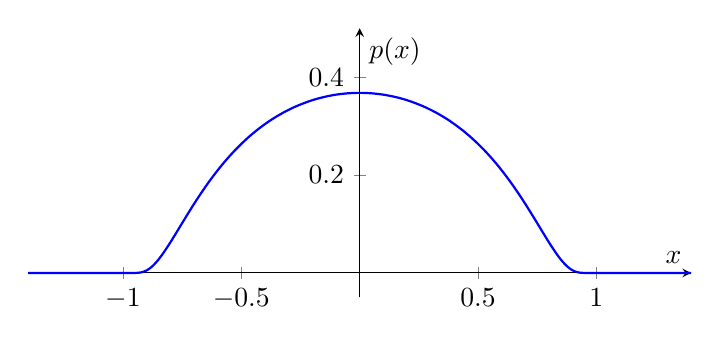
\begin{tikzpicture}
\begin{axis}[
    width=10cm, height=5cm,
    axis lines=middle,
    xlabel={$x$}, ylabel={$p(x)$},
    xmin=-1.4, xmax=1.4,
    ymin=-0.05, ymax=0.5,
    samples=300,
    domain=-1.4:1.4
]
\addplot[thick, blue]
    {abs(x)<1 ? exp(-1/(1-x^2)) : 0};
\end{axis}
\end{tikzpicture}

Let $p_\epsilon (x) := \epsilon^{-d} p(\frac{x}{\epsilon})$. Then
\[
    \int p_\epsilon(x) \; dx = \epsilon^{-d}\int p(\frac{x}{\epsilon}) \; dx
\]  
By change of variable $x' = \frac{x}{\epsilon}$, $dx' = \frac{dx}{\epsilon^d}$,
\[
    = \epsilon^{-d} \int_{\R^d} p(x') \epsilon^d \; dx' = \int_{\R^d} p(x') \; dx' = 1
\] 
And $p_\epsilon$ is supported on $B(0, \epsilon)$.

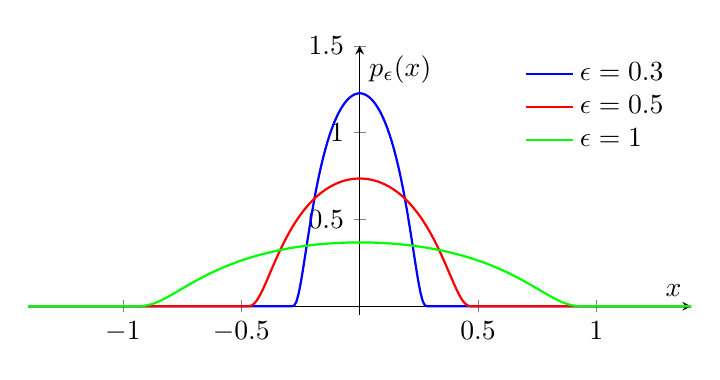
\begin{tikzpicture}
\begin{axis}[
    width=10cm, height=5cm,
    axis lines=middle,
    xlabel={$x$}, ylabel={$p_\epsilon(x)$},
    xmin=-1.4, xmax=1.4,
    ymin=-0.05, ymax=1.5,
    samples=300,
    domain=-1.4:1.4,
    legend style={at={(0.98,0.98)}, anchor=north east, draw=none, fill=none},
    legend cell align=left
]
\addplot[thick, blue]
    {abs(x/0.3)<1 ? (1/0.3)*(exp(-1/(1-(x/0.3)^2))) : 0};
\addlegendentry{$\epsilon=0.3$}

\addplot[thick, red]
    {abs(x/0.5)<1 ? (1/0.5)*(exp(-1/(1-(x/0.5)^2))) : 0};
\addlegendentry{$\epsilon=0.5$}

\addplot[thick, green]
    {abs(x)<1 ? exp(-1/(1-x^2)) : 0};
\addlegendentry{$\epsilon=1$}
\end{axis}
\end{tikzpicture}

$\{p_{\epsilon}\}_{\epsilon>0} $ is a family of "kernels" which belong to:

\begin{defn}[good kernel]
    Let $\{K_\epsilon\}_{\epsilon > 0}$ be a collection of functions s.t. $K_\epsilon : \R^d \to \R$ satisfies:
    \begin{enumerate}
        \item $\int_{\R^d} K_\epsilon(x) \; dx = 1$ for all $\epsilon > 0$
        \item $K_\epsilon \in L^1(\R^d)$ for all $\epsilon > 0$
        \item $\forall \delta > 0$, $\int_{|x| > \delta} |K_\epsilon(x)| \; dx \to 0$ as $\epsilon \to 0$. 
    \end{enumerate}  
    Then we call $\{K_\epsilon\}_{\epsilon > 0}$ a set of \newword{good kernels}. We call these kernels 
    because we will typically consider 
    \[
        f_\epsilon(x) := p_\epsilon * f = \int f(x-y)\underbrace{p_\epsilon(y) \; dy}_{\text{conv. kernel}}
    \] 
    Since $p_\epsilon \in C_c^{\infty}(\R^d)$, $\forall f \in L^p|\R^d|$, $f_\epsilon \in C^\infty(\R^d)$, 
    so $f_\epsilon$ is "smoothing $f$ out".  
\end{defn}

\begin{thm}[approximation using mollifiers]
    Let $p_\epsilon, f_\epsilon$ be as above. Then
    \begin{enumerate}
        \item If $f \in L^\infty(\R^d)$, and $f$ is continuous at $x$, then $f_\epsilon(x) \xrightarrow[\epsilon \to 0]{} f(x)$
            i.e. $f_\epsilon$ converges pointwise to $f$ at the continuity points of $f$;
            \item If $f \in C(\R^d)$, $f_\epsilon \xrightarrow[\epsilon \to 0]{} f$ uniformly on compact sets;
            \item If $f \in L^p(\R^d)$, then $f_\epsilon \xrightarrow[\epsilon \to 0]{} f$ in $L^p(\R^d)$      
    \end{enumerate} 
\end{thm}
\begin{rem}
    This is true for all good kernels $\{K_\epsilon\}_{\epsilon > 0}$ s.t. $f_\epsilon$ is well defined.
    But it is easier to redo the proof later than store a general result.
\end{rem}
\begin{proof} \leavevmode
    \begin{description}
        \item[(1)] $f$ continuous on $x$ therefore $\forall \eta > 0$, $\exists \delta > 0$
        s.t. $|x - y| < \delta \Rightarrow |f(x) - f(y)| < \eta$. So 
        \begin{align*}
            |f_\epsilon(x) - f(x)| &= \left| \int f(x-y) p_\epsilon(y) \; dy  - f(x) \right| \\
            &= \left| \int f(x-y) p_\epsilon(y) \; dy - \int f(x) p_\epsilon (y) \; dy \right| \\
            &= \left| \int (f(x-y) - f(x)) p_\epsilon \; dy \right|  \\  
            &\leq \int_{|y| \leq \delta} |f(x-y) - f(x)| p_\epsilon(y) \; dy +
            \int_{|y| > \delta} (|f(x-y)| - |f(y)|) p_\epsilon(y) \; dy \\
            &\leq \eta \int_{\R^d} p_\epsilon(y) \; dy + 2 \| f \|_\infty \int_{|y| > \delta} p_\epsilon(y) \; dy \\
            &= \eta + 2 \| f \|_\infty \int_{|y| > \delta \cap |y| < \epsilon} p_\epsilon(y) \; dy \\
        \end{align*}    
        If $\epsilon < \delta$, then $\supp(p_\epsilon) \subseteq B(0, \delta)$ so
        $\int_{|y| > \delta \cap |y| < \epsilon} p_\epsilon(y) \; dy \to 0$ as $\epsilon \to 0$,
        and thus
        \[
            \lim_{\epsilon \to 0} |f_\epsilon(x) - f(x)| \leq \eta \quad \forall \eta > 0
            \Rightarrow \lim_{\epsilon \to 0} |f_\epsilon(x) - f(x)| = 0
        \] 
        \item[(2)] If $f \in C(\R^d)$, then fix $K \subseteq \R^d $ compact. Therefore
        $f$ is uniformly continuous on $K$. So $\forall \eta > 0$, $\exists \delta > 0$ s.t.
        $|x - y| < \delta \Rightarrow \sup_{x \in K} |f(x) - f(y)| < \eta$.
        
        Also, $f \in C(\R^d)$ so 
        \[
            \frac{\sup}{K + B(0, 1)} |f(z)| \leq C
        \]
        So
        \begin{align*}
            |f_\epsilon(x) - f(x)| &\leq \int_{|y| < \delta} |f(x-y) - f(x)| p_\epsilon(y) \; dy + \int_{|y| > \delta} (|f(x-y)| + |f(x)|) p_\epsilon(y) \; dy \\
            &\leq \sup_{x \in K} \int_{|y| < \delta} |f(x-y) - f(x)| p_\epsilon(y) \; dy + \sup_{x \in K} \int_{|y| > \delta \cap |y| \leq \epsilon} (|f(x-y)| + |f(x)|) p_\epsilon(y) \; dy \\
            &\leq \eta + \frac{\sup}{K + B(0, 1)} |f(z)| \int_{|y| > \delta \cap |y| \leq \epsilon} p_\epsilon(y) \; dy \\
        \end{align*}      
        Therefore 
        \[
        \lim_{\epsilon \to 0} \sup_{x \in K} |f_\epsilon(x) - f(x)| \leq \eta \quad \forall \eta > 0 
        \]
        And thus $f_\epsilon \to f$ uniformly on $K$.   
        \item[(3)] If $f \in L^p(\R^d)$, then $\forall \eta > 0$, $\exists \tilde{f} \in C_c(\R^d)$
        s.t. 
        \[
        \| f - \tilde{f} \|_p < \eta
        \]  
        Since $\tilde{f} \in C_c(\R^d)$, $p_\epsilon$ is compactly supported, $\tilde{f_\epsilon} \in C_c^\infty(\R^d)$
        is compactly supported, so $\tilde{f_\epsilon} \to \tilde{f}$ uniformly on $\R^d$. Also,
        since $\tilde{f_\epsilon}, \tilde{f}$ are compactly supported, 
        \[
            \int |\tilde{f_\epsilon} - \tilde{f}|^p \; dx = \int_A |\tilde{f_\epsilon} - \tilde{f}|^p \; dx \leq \underbrace{\| \tilde{f_\epsilon} - \tilde{f} \|_\infty}_{\to 0 \text{ as } \epsilon \to 0} |A| 
        \]       
        Therefore $\tilde{f_\epsilon} \to \tilde{f}$ in $L^p(\R^d)$. Thus,
        \begin{align*}
            \| f_\epsilon - f \|_p &\leq \| f_\epsilon - \tilde{f_\epsilon} \|_p + \| \tilde{f_\epsilon} - \tilde{f} \|_p + \| \tilde{f} - f \|_p \\    
            &= \| (f - \tilde{f}) * p_\epsilon \|_p + \| \tilde{f_\epsilon}  - \tilde{f}\|_p + \| \tilde{f} - f \|_p \\
            &\leq \| f - \tilde{f} \|_p \| p_\epsilon \|_1 + \| \tilde{f_\epsilon} - \tilde{f} \|_p + \| \tilde{f} - f \|_p \\
            &\leq 2 \eta + \| \tilde{f_\epsilon} - \tilde{f} \|_p     
        \end{align*}  
        So, $\forall \eta > 0$,
        \[
            \lim_{\epsilon \to 0} \| f_\epsilon - f\|_p \leq 2 \eta \quad \Rightarrow f_\epsilon \to f \text{ in } L^p(\R^d) \qedhere 
        \]  
    \end{description}
\end{proof}

\begin{cor}
    $C_c^\infty(\R^d)$ is dense in $L^p(\R^d)$
\end{cor}
\begin{proof}
    By prior estimate, $\tilde{f_\epsilon} \in C_c^\infty{\R^d}$ and $\{\tilde{f_\epsilon}\}_{\epsilon > 0}$
    are dense in $L^p(\R^d)$. \qedhere   
\end{proof}

\begin{thm}[Weierstrass Approximation Theorem]
    Let $[a, b] \subseteq \R$, $f \in C([a,b])$. Then $\forall \eta > 0$, $\exists$ a polynomial
    $P$ s.t. 
    \[
        \sup_{x \in [a,b]} |f(x) - P(x)| < \eta
    \]      
    i.e. polynomials are dense in $(C([a,b]), \|\cdot\|_\infty)$.
\end{thm}
\begin{proof}
    We use a good kernel. First, for $f \in C([a,b])$, extend to $f \in C_c(\R)$.  \footnote{e.g. by linear interpolation}  
    Consider 
    \[
        K_\epsilon(x) = \frac{1}{\sqrt{\epsilon}}e^{-\frac{\pi x^2}{\epsilon}}
    \] 
    \textbf{Claim:} $\{K_\epsilon\}_{\epsilon > 0}$ is a family of good kernels.
    \newline \noindent Recall that
    \[
        \frac{1}{\sqrt{2\pi}} \int_{-\infty}^\infty e^{-\frac{x^2}{2}} \; dx = 1
    \] 
    We check:
    \begin{align*}
        \int K_\epsilon(x) \; dx &= \int \frac{1}{\sqrt{\epsilon}}e^{-\frac{\pi x^2}{\epsilon}} \; dx \\
        y = \frac{\sqrt{2\pi}}{\sqrt{\epsilon}}x &\Rightarrow dy = \frac{\sqrt{2\pi}}{\sqrt{\epsilon}}dx \\
        &= \int \frac{1}{\sqrt{\epsilon}} \frac{\sqrt{\epsilon}}{\sqrt{2\pi}} e^{-\frac{y^2}{2}} \; dy  = 1\\
    \end{align*}
    Also, 
    \[
        \int |K_\epsilon(x)| \; dx = \int K_\epsilon(x) \; dx = 1
    \] 
    Finally, we check $\forall \delta > 0$,
    \begin{align*}
        \int_{|x| > \delta} |K_\epsilon(x)| \; dx &= \int_{|x| > \delta} \frac{1}{\sqrt{\epsilon}} e^{-\frac{\pi x^2}{\epsilon}} \; dx \\
        &= \int_{|y| > \frac{\sqrt{2\pi}}{\sqrt{\epsilon}} \delta} \frac{1}{\sqrt{2\pi}} e^{-\frac{y^2}{2}} \; dy \\
        &\leq \int_{|y| \geq \frac{\sqrt{2\pi}}{\sqrt{\epsilon}} \delta} \frac{1}{\sqrt{2\pi}} |y| e^{-\frac{y^2}{2}} \; dy \\
        &= 2 \int_{\frac{\sqrt{2\pi}}{\sqrt{\epsilon}} \delta}^{\infty} \frac{1}{\sqrt{2 \pi}} r e^{-\frac{r^2}{2}} \; dr \\
        &= C e^{\frac{-r^2}{2}} \Big|_{\frac{\sqrt{2\pi}}{\sqrt{\epsilon}} \delta}^{\infty} \xrightarrow{\epsilon \to 0} 0 \\
    \end{align*}
    So $\{K_\epsilon\}$ are good kernels. Although $K_\epsilon$ is not compactly supported, 
    $f$ is compactly supported, so the same argument as in thm gives
    \[
        (f * K_\epsilon) \xrightarrow{\epsilon \to 0} f \quad \text{uniformly on } [a,b]
    \]   
    So $\exists \epsilon_0 > 0$ fixed s.t.
    \[
        \| f * K_{\epsilon_0} - f \|_{L^\infty([a,b])} < \frac{\eta}{2} \quad (*)
    \]  
    \textbf{Claim:} $\exists$ polynomial $P_N$ (of degrees $N$) s.t. $\|P_N - (f * K_{\epsilon_0})\|_{L^\infty([a,b])} < \frac{\eta}{2}$.  
    \newline \noindent Recall
    \[
        e^y = \sum_{n = 0}^\infty \frac{y^n}{n!}
    \] 
    which converges uniformly on compact sets. Define $M > 0$ s.t. 
    \[
        \sup_{x \in [a,b]} \sup_{y \in [-M, M]} |x-y| \leq M
    \]  
    So $\exists N$ s.t.
     \[
        \left\| K_{\epsilon_0}(x) - \underbrace{\frac{1}{\sqrt{\epsilon_0}} \sum_{n = 0}^N \frac{(-\frac{\pi x^2}{\epsilon_0})^n}{n!}}_{=: S_N(x)} \right\|_{L^\infty([-M, M])} < \frac{\eta}{4 M \| f \|_\infty} \footnote{Note, $S_N$ is a polynomial}
     \] 
    So $\forall x \in [a,b]$,
    \begin{align*}
        |f*K_{\epsilon_0}(x) - f*S_N(x)| &\leq \left| \int_{\R} f(x-y)(K_{\epsilon_0}(y) - S_N(y)) \; dy \right| \\
        &\leq \int_{-M}^M |f(x-y)| \left| |K_{\epsilon_0}(y) - S_N(y) \right| \; dy \\
        &\leq \| f \|_\infty \frac{\eta}{4 M \| f \|_\infty } 2M = \frac{\eta}{2}  
    \end{align*} 
    Finally, $S_N$ is a polynomial, so
    \[
        P_N(x) := (f* S_N)(x) = \int_{\R} f(y) S_N(x-y) \; dy \quad \text{ is a polynomial in } x
    \]  
    So $\forall \eta > 0$,
    \[
        \| P_N - f \|_{L^\infty([a,b])} \leq \| P_N - f * K_{\epsilon_0} \|_{L^\infty([a,b])} + \| f * K_{\epsilon_0} - f \|_{L^\infty([a,b])} < \frac{\eta}{2} + \frac{\eta}{2} = \eta \qedhere
    \]  
\end{proof}